\documentclass[10pt]{beamer}

% Packages
\usepackage{ae,lmodern}
\usepackage[utf8]{inputenc}
\usepackage[T1]{fontenc}
\usepackage[english]{babel}
\usepackage{xcolor}
\usepackage{pgfpages}
\usepackage[style=authortitle,giveninits=true,sorting=none,backend=biber]{biblatex}
\usepackage[absolute,overlay]{textpos}
\usepackage{ifdraft}
\usepackage{tikz}
\usetikzlibrary{positioning}
\usetikzlibrary{matrix}
\usetikzlibrary{arrows}
\usetikzlibrary{shapes}
\usetikzlibrary{snakes}
\usepackage{pgfplots}
% Trick to make pgfplots work with aux_dir
% (https://tex.stackexchange.com/a/444407)
% This uses the value in latexmkrc (not great, not terrible)
\pgfkeys{/pgf/plot/gnuplot call={cd build && gnuplot}}
\usepackage{amsmath,amsfonts,amsthm,bm} % Math packages
%\usepackage{mathtools} % for aligned
\usepackage{listofitems} % for \readlist to create arrays
\usepackage{stmaryrd}
\usepackage{acronym}
\usepackage{algorithm2e}
\usepackage{chronosys}

%
% General commands
%
% $Author: duboism $
% $LastChangedDate: 2011-06-21 21:26:47 +0200 (mar. 21 juin 2011) $

% TODO: better way to do that:
%  - find the current language (babel var?) and then apply a "foreign word" style
% (would work whatever the current language is)

% Latin words
\def\latinstyle{\textit}
\newcommand{\latin}[1]{\latinstyle{#1}}
\newcommand{\ie}{\latin{i.e.}}
\newcommand{\eg}{\latin{e.g.}}
\newcommand{\cf}{\latin{cf.}}
\newcommand{\etc}{\latin{etc.}}
\newcommand{\vs}{\latin{versus}}

\def\greekstyle{\textit}
\newcommand{\greek}[1]{\greekstyle{#1}}

% english words
\let\engstyle\textit
\newcommand{\english}[1]{\foreignlanguage{english}{\engstyle{#1}}}

% table titles
% TODO: better ways of doing that:
% - as an option of tabular?
% - only one command (whatever the mode)
\let\tabletitlestyle\textbf
\let\mathtabletitlestyle\mathbf
\newcommand{\tabletitle}[1]{\tabletitlestyle{#1}}
\newcommand{\mathtabletitle}[1]{\ensuremath{\mathtabletitlestyle{#1}}}

% Index
\def\indexstyle{\textbf}
\newcommand{\putindex}[1]{\indexstyle{#1}\index{#1@#1}}
\newcommand{\putindexsee}[2]{\indexstyle{#1}\index{#1@#1|see{#2}}}
\newcommand{\putindexcat}[2]{\indexstyle{#1}\index{#2@#2!{#1}}}

%
% Math commands
%
% $Author: duboism $
% $LastChangedDate: 2013-01-15 16:56:30 +0100 (mar. 15 janv. 2013) $

%\usepackage{amsmath, amssymb, amsthm, textcomp, stmaryrd}
%\usepackage{textcase}

%%%%%%%%%%%
% General %
%%%%%%%%%%%

%\newtheorem{definition}{Définition}
%\newtheorem{thm}{Théorème}
%\newtheorem{prop}{Proposition}
%\newtheorem{exemple}{Exemple}
%\newtheorem{NB}{NB}

% Sets
\def\setextleftdelim{\lbrace}
\def\setextrightdelim{\rbrace}
\newcommand{\setext}[1]{\ensuremath{\left \setextleftdelim {#1} \right \setextrightdelim}} % Ensemble en extension: {x1, ..., xn}
\def\setpredicatesep{,}
\newcommand{\setpredicate}[2]{\ensuremath{\left \setextleftdelim {#1} \setpredicatesep {#2} \right \setextrightdelim}} % Ensemble en intension: {xi, 1<= i <= n}
\def\setstyle{\mathcal}
\newcommand{\set}[1]{\ensuremath{\setstyle{#1}}}
\newcommand{\card}[1]{\ensuremath{\left | #1 \right |}}

% Well known sets
\def\setN{\mathbb{N}}
\def\setZ{\mathbb{Z}}
\def\setQ{\mathbb{Q}}
\def\setR{\mathbb{R}}
\def\setC{\mathbb{C}}

% Tuples
\def\tupleleftdelim{(}
\def\tuplerightdelim{)}
\newcommand{\couple}[2]{\ensuremath{\left \tupleleftdelim {#1}, {#2} \right \tuplerightdelim}}
\newcommand{\tupleext}[1]{\ensuremath{\left \tupleleftdelim {#1} \right \tuplerightdelim}} % Tuple en extension: (x1, ..., xn)
\def\tupleintsep{_}
\newcommand{\tupleint}[2]{\ensuremath{\left \tupleleftdelim {#1} \right \tuplerightdelim \tupleintsep {#2}}} % Tuple en intension: (xi)_{1 <= i <= n}
\def\tuplestyle{\mathbf}
\newcommand{\tuple}[1]{\ensuremath{\tuplestyle{#1}}}


% Intervals: http://en.wikipedia.org/wiki/Interval_%28mathematics%29#Notations_for_intervals
\def\intervalleftdelim{[}
\def\intervalrightdelim{]}
\def\intervallodelim{\intervalrightdelim} % left-open symbol
\def\intervalrodelim{\intervalleftdelim} % right-open symbol
\newcommand{\interval}[2]{\ensuremath{\left \intervalleftdelim {#1}, {#2} \right \intervalrightdelim}}
\newcommand{\lointerval}[2]{\ensuremath{\left \intervallodelim {#1}, {#2} \right \intervalrightdelim}}
\newcommand{\rointerval}[2]{\ensuremath{\left \intervalleftdelim {#1}, {#2} \right \intervalrodelim}}
\newcommand{\ointerval}[2]{\ensuremath{\left \intervallodelim {#1}, {#2} \right \intervalrodelim}}

% Integer intervals
\def\intintervalleftdelim{\llbracket}
\def\intintervalrightdelim{\rrbracket}
\def\intintervallodelim{\intintervalrightdelim} % left-open symbol
\def\intintervalrodelim{\intintervalleftdelim} % right-open symbol
\newcommand{\intinterval}[2]{\ensuremath{\left \intintervalleftdelim {#1}, {#2} \right \intintervalrightdelim}}
\newcommand{\lointinterval}[2]{\ensuremath{\left \intintervallodelim {#1}, {#2} \right \intintervalrightdelim}}
\newcommand{\rointinterval}[2]{\ensuremath{\left \intintervalleftdelim {#1}, {#2} \right \intintervalrodelim}}
\newcommand{\ointinterval}[2]{\ensuremath{\left \intintervallodelim {#1}, {#2} \right \intintervalrodelim}}

% Functions and operators
\def\functionstyle{\mathrm}
\newcommand{\func}[1]{\ensuremath{\functionstyle{#1}}}
\newcommand{\apply}[2]{\ensuremath{#1 \left ( {#2} \right )}}
\def\opstyle{\mathrm}
\newcommand{\op}[1]{\ensuremath{\opstyle{#1}}}
\newcommand{\applyop}[2]{\ensuremath{#1 \left [ {#2} \right ]}}

% Vectors, Matrices, ...
\def\vectorextleftdelim{[}
\def\vectorextrightdelim{]}
\newcommand{\vectorext}[1]{\ensuremath{\left \vectorextleftdelim {#1} \right \vectorextrightdelim}}
\newcommand{\vectorstyle}[1]{\mathbf{#1}}
\renewcommand{\vector}[1]{\ensuremath{\vectorstyle{#1}}}
\newcommand{\vectorElem}[2]{\ensuremath{#1 \left [ #2 \right ]}}

\def\matrixextleftdelim{[}
\def\matrixextrightdelim{]}
\newcommand{\matrixext}[1]{\ensuremath{\left \matrixextleftdelim {#1} \right \matrixrightdelim}}
\def\matrixstyle{\mathbf}
\renewcommand{\matrix}[1]{\ensuremath{\matrixstyle{#1}}}
\newcommand{\matrixElem}[3]{\ensuremath{#1 \left [ {#2}, {#3} \right ]}}
\newcommand{\matrixLinElem}[2]{\ensuremath{#1 \left [ #2 \right ]}}

% Scalar product
\def\dotprodleftdelim{\left \langle}
\def\dotprodrightdelim{\right \rangle}
\def\dotprodcentraldelim{,}
\newcommand{\dotprod}[2]{\ensuremath{\dotprodleftdelim #1 \dotprodcentraldelim #2 \dotprodrightdelim}}

% Vector product
\def\vectorprodsymbol{\times}
\newcommand{\vectorprod}[2]{#1 \vectorprodsymbol #2}

% TODO:
% - sets: set builder notation? http://en.wikipedia.org/wiki/Set_builder_notation
% - set theory: define synonyms for common opertaions (union <-> \bigcup, intersection <-> \bigcap, etc.)
% - matrix
% - indexing should be done on class basis: setelement, matrix element, imageelement, ...
% - limits: use \def instead of \newcommand?
% - probabilities: use \DeclareMathOperator? There is a \Pr operator in \LaTeX

% Integral
\def\dsymb{\mathrm{d}}
\newcommand{\intover}[1]{\dsymb #1}

% Limits
\newcommand{\tendsto}[1]{\ensuremath{\rightarrow #1}}
\newcommand{\tendstoP}{\ensuremath{\overset{P}{\rightarrow}}}

% Optimal quantity
\def\optsymbol{\star}
\newcommand{\opt}[1]{\ensuremath{\overset{\optsymbol}{#1}}}

% Estimation of a quantity
\def\estimsymbol{\widehat}
\newcommand{\estim}[1]{\ensuremath{\estimsymbol{#1}}}

%%%%%%%%%%%%%%%%%
% Probabilities %
%%%%%%%%%%%%%%%%%
\newcommand{\RV}[1]{\ensuremath{\MakeTextUppercase{#1}}}
\newcommand{\cond}[2]{{#1} | {#2}}


% Discrete probability
\def\probSymbol{P}
\newcommand{\prob}[1]{\ensuremath{\apply{\func{\probSymbol}}{#1}}}
\newcommand{\condprob}[2]{\ensuremath{\prob{\cond{#1}{#2}}}}

% PDF
\def\pdfSymbol{p}
\newcommand{\pdf}[1]{\ensuremath{\apply{\func{\pdfSymbol}}{#1}}}
\newcommand{\condpdf}[2]{\ensuremath{\pdf{\cond{#1}{#2}}}}

% Operators
\newcommand{\expectation}[1]{\ensuremath{\applyop{\op{\mathbb{E}}}{#1}}}
\newcommand{\var}[1]{\ensuremath{\applyop{\op{Var}}{#1}}}


%%%%%%%%%%%%%%%%%%%%%%
% General operations %
%%%%%%%%%%%%%%%%%%%%%%

% Argmax & friends
\DeclareMathOperator*{\argmax}{arg\,max}
\DeclareMathOperator*{\argmin}{arg\,min}

% BigO and friends
% From: http://www.tug.org/pipermail/texhax/2004-January/001496.html
% See also: http://xw2k.nist.gov/dads//HTML/bigOnotation.html
\DeclareMathOperator{\BigOmicron}{O}
\DeclareMathOperator{\littleomicron}{o}
\DeclareMathOperator{\BigOmega}{\Omega}
\DeclareMathOperator{\littleomega}{\omega}
\DeclareMathOperator{\BigTheta}{\Theta}

\newcommand{\boundedabove}[1]{\BigOmicron \left ( {#1} \right )}
\newcommand{\dominated}[1]{\littleomicron \left ( {#1} \right )}

\newcommand{\boundedbelow}[1]{\BigOmega \left ( {#1} \right )}
\newcommand{\dominates}[1]{\littleomega \left ( {#1} \right )}

\newcommand{\boundedabovebelow}[1]{\BigTheta \left ( {#1} \right )}
\newcommand{\similar}[2]{{#1} \sim {#2}}

% Norms
\def\normleftdelim{\|}
\def\normrightdelim{\|}
\newcommand{\pnorm}[2]{\ensuremath{\left \normleftdelim {#1} \right \normrightdelim_{#2}}}
\newcommand{\norm}[1]{\ensuremath{\left \normleftdelim {#1} \right \normrightdelim}}
\newcommand{\abs}[1]{\ensuremath{\left | {#1} \right |}}

% Special functions
\newcommand{\ceil}[1]{\ensuremath{\left \lceil {#1} \right \rceil}}
\newcommand{\floor}[1]{\ensuremath{\left \lfloor {#1} \right \rfloor}}
\DeclareMathOperator{\sgn}{sgn}

% Convolution
\def\convsymbol{\star}
\DeclareMathOperator*{\conv}{\convsymbol}
\newcommand{\convvar}[1]{\ensuremath{\conv_{#1}}} % argument is used to specify convolution variables

%%%%%%%%%%%%%%%%%%%%
% Image processing %
%%%%%%%%%%%%%%%%%%%%

\let\imagestyle\mathbf
\newcommand{\image}[1]{\ensuremath{\imagestyle{#1}}}
\newcommand{\imagepixel}[3]{\ensuremath{\image{#1} \left ( #2, #3 \right )}}
\newcommand{\gausskernel}[3]{\ensuremath{\frac{1}{\sqrt{2\pi} #3} \exp^{-\frac{(#1+#2)^2}{2 #3^2}} }}

% SIFT
\newcommand{\siftkernel}{\gausskernel{x}{y}{\sqrt{2}}}

%\newcommand{\convdd}[4]{\int_3 \int_4 #1 #2}

%%%%%%%%%%%%
% Learning %
%%%%%%%%%%%%

\DeclareMathOperator{\error}{error}

% Probabilistic robotics
\newcommand{\stateSymbol}{x}
\newcommand{\state}{\vector{\stateSymbol}}
\newcommand{\obsSymbol}{z}
\newcommand{\obs}{\vector{\obsSymbol}}
\newcommand{\controlSymbol}{u}
\newcommand{\control}{\vector{\controlSymbol}}
\newcommand{\aggState}{\tilde{x}}
\newcommand{\stateRVSymbol}{\RV{\stateSymbol}}
\newcommand{\stateRV}{\vector{\stateRVSymbol}}
\newcommand{\obsRVSymbol}{\RV{\obsSymbol}}
\newcommand{\obsRV}{\vector{\obsRVSymbol}}
\newcommand{\controlRVSymbol}{\RV{\controlSymbol}}
\newcommand{\controlRV}{\vector{\controlRVSymbol}}
\newcommand{\aggStateRV}{\RV{\aggState}}

\newcommand{\val}[2]{\ensuremath{{#1}_{#2}}}
\newcommand{\seq}[3]{\ensuremath{{#1}_{{#2}:{#3}}}}

\newcommand{\bel}{\func{bel}}
\newcommand{\belBeforeObs}{\overline{{\bel}}}



% Options, definitions and styles
%\setbeameroption{show notes on second screen}
\DeclareFontShape{T1}{cmss}{b}{n}{<->ssub * cmss/bx/n}{}
\AtBeginSection[]{%
  \begin{frame}
    \frametitle{Outline}
    \tableofcontents[currentsection,hideothersubsections]
  \end{frame}
}
\AtBeginSubsection[]{%
  \begin{frame}
    \frametitle{Outline}
    \tableofcontents[currentsection,subsectionstyle=show/shaded/hide]
  \end{frame}
}
% Grid
\TPGrid{100}{100}
\ifdraft
  {%
    \TPoptions{%
      showboxes=true,%
    }%
  }%
  {%
  }
% Hyperref
\hypersetup{
  colorlinks=true,
  linkcolor=blue,
  filecolor=magenta,
  urlcolor=cyan,
}
% TiKz
\tikzset{%
  every neuron/.style={
    circle,
    draw,
    %minimum size=1cm
  },
  neuron missing/.style={
    draw=none,
    scale=2.5,
    text height=0.333cm,
    execute at begin node=\color{black}$\vdots$
  },
}
% Bibliography and citation style
\addbibresource{references.bib}
\DeclareNameAlias{author}{last-first}
\DeclareBibliographyCategory{AI}
\addtocategory{AI}{stuart2021}
\DeclareBibliographyCategory{ML}
\addtocategory{ML}{bishop2006}
\addtocategory{ML}{duda2001}
\addtocategory{ML}{james2023}
\addtocategory{ML}{barra2021}
\DeclareBibliographyCategory{deep_learning}
\addtocategory{deep_learning}{goodfellow2016}
\addtocategory{deep_learning}{zhang2023}
\addtocategory{deep_learning}{chollet2021}

% Notations

% Examples
\def\exampleSet{\set{X}}
\def\pdfExample{\pdfSymbol_{\exampleSet}}
\def\example{\vector{x}}
\def\dimExample{d}

% Labels
\def\labelSet{\set{Y}}
\def\condpdfLabelExample{\pdfSymbol_{\labelSet | \exampleSet}}
\def\knownLabel{u}
\def\predLabel{y}
\def\nClasses{K}

\def\pdfExampleLabel{\pdfSymbol_{\exampleSet \labelSet}}

% Training set
\def\trainingSet{\set{S}}
\def\nTrainingSamples{m}

\def\targetFunc{\func{f}}
\def\hypSet{\set{H}}
\def\hyp{\func{h}}
\def\params{\vector{\theta}}

\def\risk{\func{R}}
\def\empRisk{\func{R_{emp}}}

% For NN
\def\output{o}
\def\layer{\ell}
\def\weight{w}
\def\weightMatrix{\matrix{W}}
\def\activFunc{\func{\sigma}}
\def\ReLUFunc{\func{ReLU}}
\def\ReLUFuncExt{\func{\max}}
\def\softMaxFunc{\func{SoftMax}}
\def\lossFunc{\func{L}}
\def\learningRate{\alpha}
\DeclareMathOperator{\grad}{\nabla}

% Acronyms
\acrodef{AI}{Artificial Intelligence}
\acrodef{xAI}{eXplainable AI}
\acrodef{ML}{Machine Learning}
\acrodef{NN}{Neural Networks}
\acrodef{DL}{Deep Learning}
\acrodef{MLP}{Multi-Layer Perceptron}
\acrodef{CNN}{Convolutional Neural Networks}

\title{Introduction to Machine Learning}
\author{Sylvain Caillou \and Mathieu Dubois}
\institute{MaNiTou 2024}
\date{2024-07-05}

\begin{document}

\frame{\titlepage}


\begin{frame}
  \note{
    \begin{itemize}
    \item Limits and approach of our talk
      \begin{itemize}
      \item At the end you should be able to understand the first lines of
        \acs{ML} articles
      \end{itemize}
    \item Introduce Natalia's talk
    \end{itemize}
  }
  \frametitle{Goal}

  \begin{textblock}{90}(5, 15)
    \begin{itemize}
    \item \aclu{ML} is a vast and expanding universe \onslide<2->{with $\Lambda
        > 0$}
    \item<3-> We can't talk about everything:
      \begin{itemize}
      \item<4-> We will start with a simple example and then generalize
      \item<4-> We won't talk much about GW
      \end{itemize}
    \item<5-> Next talk will introduce more advanced models in the context of GW
    \end{itemize}
  \end{textblock}
\end{frame}


\begin{frame}
  \frametitle{Outline}
  \tableofcontents[hidesubsections]
\end{frame}

\section{Introduction}

\subsection{Definition \& history}

\begin{frame}
  \note{
    \begin{itemize}
    \item Ask them a few hints
    \item Talk about definitions
    \item $DL \subset ML \subset AI$:
      \begin{itemize}
      \item \acs{DL} is sometimes used as a synonym for \acs{AI}
      \item this inclusion hides the rich connection between the fields
      \end{itemize}
    \end{itemize}
  }
  \frametitle{Definition of \acs{AI} and \acs{ML}}

  \begin{textblock}{90}(05,15)
    \begin{itemize}
    \item<2-> \acf{AI}:
      \begin{itemize}
      \item Discipline focused on creating systems capable of
        performing tasks that typically require human intelligence, such as
        problem-solving, decision-making, translation, \etc{}
      \end{itemize}
    \item<3-> \acf{ML}:
      \begin{itemize}
      \item Field of \ac{AI} focused on the development and study
        of systems that can ``learn from experience''.
      \item<4-> ``A system is said to learn from experience
        E with respect to some class of tasks T and performance measure P if
        its performance at tasks in T, as measured by P, improves with
        experience E'' (Tom Mitchell).
      \end{itemize}
    \item<5-> \acf{DL}:
      \begin{itemize}
      \item Field of \ac{ML} concerned with a certain class of
      models
      \item Better definition later
      \end{itemize}
    \item<6-> \ac{DL} $\subset$ \ac{ML} $\subset$ \ac{AI}:
      \begin{itemize}
      \item \ac{ML} (particularly \ac{DL}) is a necessary ingredient of \ac{AI}
        but it's not the end of the story
      \end{itemize}
    \end{itemize}
  \end{textblock}

\end{frame}


\begin{frame}
  \note{
    \begin{itemize}
    \item Phases
    \item Brief overview of the beginning:
      \begin{itemize}
      \item Lot of ideas (link with cognitive science, logic, information
        theory, cybernetics \etc{}) \& concrete realizations (functional and OO
        languages, algorithms, CAS, \etc{})
      \item Herbert Simon (1958): ``Within ten years a digital computer will be
        the world's chess champion''
      %\item John McCarthy: ``As soon as it works, nobody calls it \ac{AI} anymore''
      \end{itemize}
    \item Winters
      \begin{itemize}
      \item Lighthill report (1973): ``In no part of the field have the
        discoveries made so far produced the major impact that was then
        promised''
      \item Kasparov \vs{} Deep Blue (1997): nothing to do with \ac{ML}
      \end{itemize}
    \item Rise of ML:
      \begin{itemize}
      \item Practical causes
      \end{itemize}
    \item Rise of DL:
      \begin{itemize}
      \item NN are mature
      \end{itemize}
    \end{itemize}
  }
  \frametitle{A brief history of \acs{AI} and \acs{ML}}

  \begin{textblock}{90}(05,10)
    % Display history with or without dates
    \def\historyOverview{
      \chronoperiode[color=black,startdate=false,stopdate=false]{1950}{1955}{
        % Pre-history
      }
      \chronoperiode[color=white,startdate=false,stopdate=false]{1955}{1956}{
        % Empty period
      }
      \chronoperiode[textstyle=\rotatebox{45},textdepth=39pt,color=purple,datesstyle=\showDates]{1956}{1973}{
        Beginning
      }
      \chronoperiode[textstyle=\rotatebox{45},textdepth=43pt,color=lightgray,datesstyle=\showDates]{1973}{1980}{
        1st winter
      }
      \chronoperiode[textstyle=\rotatebox{45},textdepth=39pt,color=lightgray,datesstyle=\showDates]{1987}{2000}{
        2nd winter
      }
      \chronoperiode[textstyle=\rotatebox{45},textdepth=40pt,color=orange,datesstyle=\showDates]{2000}{2012}{
        Rise of \ac{ML}
      }
      \chronoperiode[textstyle=\rotatebox{45},textdepth=40pt,color=red,datesstyle=\showDates]{2012}{2024}{
        Rise of \ac{DL}
      }
    }
    \only<1>{
      \begin{chronology}[startyear=1950,stopyear=2024,height=1cm,startdate=false,stopdate=false]
        \def\showDates{\color{white}}
        \historyOverview
      \end{chronology}
    }
    \onslide<2->{
      \begin{chronology}[startyear=1950,stopyear=2024,height=1cm,startdate=false,stopdate=false]
        \def\showDates{}
        \historyOverview
      \end{chronology}
    }
  \end{textblock}

  \begin{textblock}{45}(05,45)
    \begin{itemize}
    \item<2-> Beginning
      \begin{itemize}
      \item \ac{AI}: Dartmouth workshop (1956)
      \item<3-> \ac{ML}: Arthur Samuel (1959)
      \item<4-> MANY approaches, techniques (including \acs{NN}), realizations
        and hopes
      \end{itemize}
    \item<5-> Some ideas didn't work in the real world:
      \begin{itemize}
      \item ``Winters'' of \ac{AI}
      \item<6-> Development never halted
      \end{itemize}
    \end{itemize}
  \end{textblock}

  \begin{textblock}{45}(50,45)
    \begin{itemize}
    \item<7-> Rise of \ac{ML} at the turn of the millennium
      \begin{itemize}
      \item Built on work of previous decades
      \item Lots of data, processing and storage capability, mature technology
      \end{itemize}
    \item<8-> Rise of \acl{DL} since 2012
      \begin{itemize}
      \item AlexNet (2012): first \ac{DL} model to out-performs other \ac{ML}
        methods
      \item More on that in the last section
      \end{itemize}
    \end{itemize}
  \end{textblock}
\end{frame}


% Benefits/risks of ML
\begin{frame}
  \note{
    \begin{itemize}
    \item Present benefits and risks
    \item Almost each benefit as a potential counterpart
    \end{itemize}
  }
  \frametitle{Benefits and risks of \ac{ML}}

  \begin{textblock}{45}(5, 15)
    \begin{block}{Benefits}
      % Large scale deployment of \ac{ML} technology could benefit to:
      \begin{itemize}
      \item Deeper understanding of some phenomena:
        \begin{itemize}
        \item Prediction, classification, \etc{}
        \item Quantitative approach (Social Sciences, \etc{})
        \item Better modelling
        \end{itemize}
      \item Better services:
        \begin{itemize}
        \item Personalized medecine, smart cities, smart grids, \etc{}
        \item Personal assistant
        \end{itemize}
      \end{itemize}
    \end{block}
  \end{textblock}

  \begin{textblock}{45}(50, 15)
    \begin{block}{Risks}<2->
      % Large scale deployment of \ac{ML} technology could be detrimental to:
      \begin{itemize}
      \item Ethical/Political aspects:
        \begin{itemize}
        \item Blind decision
        \item Discrimination
        \item Manipulation
        \end{itemize}
      \item Legal aspects:
        \begin{itemize}
        \item Privacy, safety, security, copyrights
        \end{itemize}
      \item Cognitive effects:
        \begin{itemize}
        \item Loss of skills
        \item Attention span
        \end{itemize}
      \item Economical aspects:
        \begin{itemize}
        \item Disappearance of some jobs
        \item Over-importance of some companies
        \end{itemize}
      \item Environmental impact
      \end{itemize}
    \end{block}
  \end{textblock}
\end{frame}


\subsection{How to go further?}

\begin{frame}
  \note{
    \begin{itemize}
    \item Here are the most important slides
    \end{itemize}
  }
  \frametitle{General books}

  \nocite{*}

  \begin{textblock}{90}(5, 15)
    \begin{block}{AI}<1->
      \printbibliography[heading=none,category=AI]
    \end{block}

    \begin{block}{\ac{ML}}<2->
      \printbibliography[heading=none,category=ML]
    \end{block}
  \end{textblock}
\end{frame}

\begin{frame}
  \frametitle{Deep learning books}

  \nocite{*}

  \begin{textblock}{90}(5, 15)
    \begin{block}{DL}<1->
      \printbibliography[heading=none,category=deep_learning]
    \end{block}
  \end{textblock}
\end{frame}

\begin{frame}
  \frametitle{Courses \& tutorials}

  \begin{textblock}{90}(5, 15)
    \begin{block}{Courses}<1->
      \begin{itemize}
      \item Coursera MOOC:
        \url{https://www.coursera.org/specializations/machine-learning-introduction} (more or less based on \href{https://cs230.stanford.edu/}{Stanford CS230 (Deep Learning)})
      \item FIDLE (Formation Introduction au Deep LEarning): \url{https://fidle.cnrs.fr/}
        (yearly course with practical examples in French)
      \end{itemize}
    \end{block}

    \begin{block}{Hands-on}<2->
      \begin{itemize}
      \item Challenges:
        \begin{itemize}
        \item Kaggle: \url{https://www.kaggle.com/}
        \item ENS Challenge Data: \url{https://challengedata.ens.fr/}
        \end{itemize}
      \item Tutorials
        \begin{itemize}
        \item PyTorch tutorials: \url{https://pytorch.org/tutorials/}
        \item scikit-learn tutorials:
          \url{https://scikit-learn.org/stable/user_guide.html}
        \end{itemize}
      \end{itemize}
    \end{block}
  \end{textblock}
\end{frame}


\section[A simple example: MLP]{A simple example: classify handwritten digits with a \acl{MLP}}

\begin{frame}
  \note{
    \begin{itemize}
      \item Explain why we will talk about the MLP
    \end{itemize}
  }

  \frametitle{\acl{MLP}: Introduction}

  \begin{textblock}{80}(5, 20)
    \begin{itemize}
    \item<1-> First perceptrons (introduced in 1957) were very limited
      \begin{itemize}
      \item Many improvements since: hidden layers and activation functions
      \item Lots of variations
      \end{itemize}
    \item<1-> Loose biological inspiration
    \end{itemize}
  \end{textblock}
\end{frame}


\begin{frame}
  \note{
    \begin{itemize}
    \item Classification task
    \item Supervised learning
    \item Preprocessing
    \item Split test-train
    \end{itemize}
  }

  \frametitle{The MNIST dataset}

  \begin{columns}
    \begin{column}{0.5\textwidth}
      \begin{itemize}
      \item Classic dataset:
        \begin{itemize}
        \item Lots of methods have been tested with it
        \end{itemize}
      \item<2-> The task is to recognize the digit on the image
        % \ie{} we are looking
        % for a function: $\hyp: \, \setR^{\dimExample} \mapsto
        % \intinterval{0}{9}$
        \begin{itemize}
          \item Classification
        \end{itemize}
      \item<3-> Train set: 60 000 images
        \begin{itemize}
        \item $\trainingSet =
          \setpredicate{\couple{\example_{i}}{\knownLabel_{i}}}{i=1..\nTrainingSamples}$
        \item $\example_i \in \setR^{\dimExample}, \dimExample = 784$
        \item $\knownLabel_i \in \intinterval{0}{9}$
        \end{itemize}
      \item<3-> Test set: 10 000 images
      \item<4-> Pre-processing:
        \begin{itemize}
        \item All images have the same size ($28 \times 28$)
        \item Centered around center of mass of the pixels
        \end{itemize}
      \end{itemize}
    \end{column}
    \begin{column}{0.5\textwidth}
      \begin{tikzpicture}[>=stealth]
        \node[anchor=south west,inner sep=0] (image) at (0,0) {
          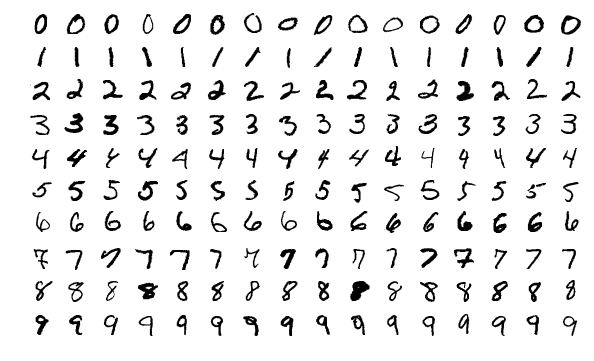
\includegraphics[width=\columnwidth]{img/MnistExamples.png}
        };
        \onslide<2->{
        \begin{scope}[x={(image.south east)},y={(image.north west)}]
          \draw[red,ultra thick] (0.22,0.15) rectangle (0.28,0.25);
        \end{scope}
        }
      \end{tikzpicture}
      \url{http://yann.lecun.com/exdb/mnist/index.html}
    \end{column}
  \end{columns}
\end{frame}


\subsection{How does it work?}

\begin{frame}
  \note{
    \begin{itemize}
    \item Probabilistic classifier:
      \begin{align*}
        \begin{aligned}
          & \hyp_{\params} : & \setR^{\dimExample} & \rightarrow & \interval{0}{1}^{\nClasses} \\
        \end{aligned}
      \end{align*}
      where
      $\vector{\predLabel} = \apply{\hyp_{\params}}{\example}$ is a vector such
      that $\vectorElem{\vector{\predLabel}}{k}$ is $\prob{\example = k}$
    \item Feed-forward
    \item Parametrized function
    \item Importance of non-linear activation function
    \item Note that we neglected bias term
    \item Idea:
      \begin{itemize}
      \item Hidden layers learn internal representations of the data
      \end{itemize}
    \end{itemize}
  }

  \frametitle{\acl{MLP}: Computation}
  \begin{textblock}{100}(5,15)
    \begin{tikzpicture}[>=stealth]
      % Inspired by https://tex.stackexchange.com/a/153974
      % We display a MLP with 2 hidden layers for OCR
      % The input image and the output layer are always displayed
      % The layers (input and the 2 hidden) and their connections appear after
      % Description of layers are on the graph
      % The number of neurons per layer is taken from
      % Gradient-Based Learning Applied to Document Recognition, Le Cun et al., 1998

      % Parameters
      \def\xInputImage{0}
      \def\nameInputImage{input-name}
      \def\xInput{2.0}
      \def\nameInput{input}
      \def\xHiddenI{4.3}
      \def\nameHiddenI{hidden1}
      \def\xHiddenII{6.6}
      \def\nameHiddenII{hidden2}
      \def\xOutput{8.9}
      \def\nameOutput{output}
      \def\xProba{9.4}
      \def\nameProba{proba}
      \def\missing{missing}

      % Input image and grid
      % This part is inspired by https://tex.stackexchange.com/a/128648
      % and a lot of trial and error for the grid (including a bit of ChatGPT)
      % Apparently, the idea is to fix the size of the image and then the grid
      % flows
      % I use 56px (twice the real size) so that it looks OK and computations are easy.
      \node[anchor=center,inner sep=0pt,draw=black] (\nameInputImage) at (\xInputImage,0) {
        
\includegraphics[width=56px,height=56px]{img/Mnist_8.png}
      };
      \begin{scope}
        \clip (\nameInputImage.south west) rectangle (\nameInputImage.north east);
        \draw[step=2px,gray,very thin] (\nameInputImage.south west) grid (56px, 56px);
      \end{scope}

      \onslide<2->{
      % Input layer
      \node [align=center, above] at (\xInput,2.2) {%Input \\ layer \\
          {\tiny $28\times28=784$ units}};
      \foreach \m/\l [count=\y] in {1,2,3,missing,784}
      \node [every neuron/.try, neuron \m/.try] (\nameInput-\m) at (\xInput,3.0-\y) {};

      % Connections from input image to input layer
      % No loop here cause we need to shift the positions
      % It uses the scale introduced above
      \draw [->] (\nameInputImage)++(-27px,27px) -- (\nameInput-1);
      \draw [->] (\nameInputImage)++(-25px,27px) -- (\nameInput-2);
      \draw [->] (\nameInputImage)++(-23px,27px) -- (\nameInput-3);
      \draw [->] (\nameInputImage)++(27px,-27px) -- (\nameInput-784);
      }

      % Description of the output
      \onslide<2>{
      \node[text width=3cm,anchor=north west] at (\xInput-1, -2.2) {{\footnotesize
          $\output^{1}_{k} = \vectorElem{\example}{k}$
      }} ;
      }

      % Matrix form
      \onslide<3->{
      \node[text width=3cm,anchor=north west] at (\xInput-1, -2.2) {{\footnotesize
          $\vector{\output}^{1} = \example$
      }} ;
      }

      % First hidden layer
      % Connections are displayed in 2 different slides (see below)
      \onslide<3->{
      \node [align=center, above] at (\xHiddenI,2.2) {%Hidden \\ layer \\
          {\tiny 300 $\ReLUFunc$ units}};
      \foreach \m [count=\y] in {1,2,missing,3}
      \node [every neuron/.try, neuron \m/.try ] (\nameHiddenI-\m) at (\xHiddenI,2.5-\y) {};
      }

      % Connections from input layer to first neuron with weights
      % and explanation of the output
      \onslide<3>{
      \foreach \p in {1,2,3,784}
      \foreach \k in {1}
      \draw[->] (\nameInput-\p) -- node {${\color{red} \weight^{1}_{\k,\p}}$} (\nameHiddenI-\k);

      % Description of the output
      \node[text width=3cm,anchor=north west] at (\xHiddenI-1, -2.2) {{\footnotesize
          $s^{2}_{k} = \sum_{p=1}^{N_{1}} {\color{red} \weight^{1}_{k,p}} \output^{1}_{p} $
      }};
      \node[text width=5cm,anchor=north west] at (\xHiddenI-1, -3.0) {{\footnotesize
          $\output^{2}_{k} = \apply{\ReLUFuncExt}{0, s^{2}_{k}}$ ($\ReLUFunc$)
      }};
      }

      % Other connections from input layer to first hidden layer
      % and matrix form
      \onslide<4->{
      \foreach \i in {1,2,3,784}
      \foreach \j in {1,...,3}
      \draw[->] (\nameInput-\i) -- (\nameHiddenI-\j);
      \node[text width=3cm,anchor=north west] at (\xHiddenI-1.2, -2.2) {{\footnotesize
          $\vector{\output^{2}} = \apply{\ReLUFunc}{{\color{red}\weightMatrix^{1}}\vector{\output^{1}}}$
      }};
      }

      % Second hidden layer
      \onslide<5->{
      \node [align=center, above] at (\xHiddenII,2.2) {% Hidden \\ layer \\
          {\tiny 100 $\ReLUFunc$ units}};
      \foreach \m [count=\y] in {1,2,missing,3}
      \node [every neuron/.try, neuron \m/.try ] (\nameHiddenII-\m) at (\xHiddenII,2.2-0.9*\y) {};

      % Connections to first hidden layer to second hidden layer
      \foreach \i in {1,2,3}
      \foreach \j in {1,2,3}
      \draw [->] (\nameHiddenI-\i) -- (\nameHiddenII-\j);

      \node[text width=3cm,anchor=north west] at (\xHiddenII-1, -2.4) {{\footnotesize
          $\vector{\output^{3}} = \apply{\ReLUFunc}{{\color{red}\weightMatrix^{2}}\vector{\output^{2}}}$
      }};
      }

      % Output layer
      \node [align=center, above] at (\xOutput,2.2) {% Output \\ layer \\
        {\tiny 10 $\softMaxFunc$ units}};
      \foreach \m [count=\y] in {0,1,missing,9}
      \node [every neuron/.try, neuron \m/.try ] (\nameOutput-\m) at (\xOutput,1.6-0.7*\y) {};

      \onslide<6->{
      % Connection from second hidden layer to output layer
      \foreach \i in {1,2,3}
      \foreach \j in {0,1,9}
      \draw [->] (\nameHiddenII-\i) -- (\nameOutput-\j);
      }

      % Description of output
      \onslide<6>{
      \node[text width=3cm,anchor=north west] at (\xOutput-0.5, -2.2) {{\footnotesize
          $s^{4}_{k} = \sum_{p=1}^{N_{3}} {\color{red} \weight^{3}_{k,p}} \output^{3}_{p}$
      }};
      \node[text width=5cm,anchor=north west] at (\xOutput-0.5, -3.0) {{\footnotesize
          $\output^{4}_{k} = \frac{\apply{\exp}{s^{4}_{k}}}{\sum_{j=1}^{10} \apply{\exp}{s^{4}_{j}}}$
      }};
      }

      \onslide<7->{
      \node[text width=3cm,anchor=north west] at (\xOutput-0.7, -2.2) {{\footnotesize
          $\vector{\output^{4}} = \apply{\softMaxFunc}{{\color{red}\weightMatrix^{3}}\vector{\output^{3}}}$
      }};
      }


      % Output probabilities
      \foreach \m [count=\y] in {0,1,missing,9}
      \node (\nameProba-\m) at (\xProba,1.6-0.7*\y) {\ifx\m\missing\else {\tiny $\prob{\m}$}\fi};

      % Description (put above for clarity)
      \onslide<7->{
      \node[text width=10cm,anchor=north west] at (-1, 3.5) {{\footnotesize
          \acsu{MLP} is a parametrized function $\hyp_{\params}$ where
          ${\color{red}\params}$ is the vector containing the {\tiny $784 \times
          300 + 300 \times 100 + 100 \times 10 = $} 266 200 weights
      }};
      }
    \end{tikzpicture}

  \end{textblock}

\end{frame}


\subsection{Learning}

\begin{frame}
  \frametitle{\acl{MLP}: Learning (1/2)}

  \begin{block}{Goal}
    Adjust $\params$ to give a better performance
  \end{block}

  \begin{block}{General idea}<2->
    %Bad prediction: $\predLabel_i =
    %\apply{\hyp_\params}{\example_i}$ is far from $\knownLabel_i$
    \begin{itemize}
    \item<2-> Define a loss function $\lossFunc$ such that $\apply{\lossFunc}{
            \apply{\hyp_\params}{\example_i},
            \knownLabel_i
          }$ is high if $\apply{\hyp_\params}{\example_i}$ is far from
          $\knownLabel_i$
     \item<3-> Minimize $\lossFunc$ (as a function of $\params$)
     \item<4-> The correct loss function depends on the problem
    \end{itemize}
  \end{block}

  \begin{block}{In our example}<5->
    \begin{itemize}
    \item $\predLabel_i = \apply{\hyp_\params}{\example_i}$ is a vector $\vectorext{\prob{0}, \prob{1}, \cdots,
        \prob{8}, \prob{9}}^T$
    \item $u_i$ is the label \onslide<6->{$\rightarrow$ transform it $\vectorext{0, 0, \cdots, 1, 0}^T$ (one-hot
      encoding)}
  \item<7-> Cross-entropy loss:
    \begin{center}
      $
        \apply{\lossFunc}{\apply{\hyp_\params}{\example_i},
          \knownLabel_i} = \only<7>{- \sum_{c=1}^{10} \vectorElem{u_i}{c}
          \apply{\log}{\vectorElem{\predLabel_i}{c}}}
                           \only<8->{- \apply{\log}{\prob{8}}}
      $
    \end{center}
    \item<9-> Cross-entropy is more general
    \end{itemize}
  \end{block}
\end{frame}


\begin{frame}[label=MLP_learning_2]
  \frametitle{\acl{MLP}: Learning (2/2)}

  \begin{textblock}{45}(5,15)
    \begin{block}{How to minimize $\lossFunc$?}
      \onslide<2->{
        If we know the gradient of $\lossFunc$ at $\params_{t}$ we can update:
        \[
          \params_{t+1} \leftarrow \params_{t} - \learningRate
          \apply{\grad_{\params}\lossFunc}{\params_{t}}
        \]
      }
    \end{block}
  \end{textblock}

  % Cheat a bit on the position
  \begin{textblock}{50}(50,12)
    \begin{center}
    \begin{tikzpicture}[domain=0:4,yscale=0.8]
      % Display a 1-D analytical loss function (x-2)**2 + 0.3
      % to illustrate
      \def\paramsInit{3} % Current value of the parameter
      \def\lossInit{1.3} % Current value of the loss
      \def\gradVal{2}    % Value of the gradient

      % \draw[very thin,color=gray] (-0.1,-0.1) grid (3.9,3.9);
      \draw[->] (-0.2,0) -- (4.2,0) node[right] {$\params$};
      \draw[->] (0,-0.2) -- (0,4.2) node[above right] {$\apply{\lossFunc}{\apply{\hyp_{\params}}{\example_i}, \knownLabel_i}$};
      % Display loss function
      \draw[color=blue] plot function{(x-2)**2+0.3} node[right] {};

      % Value at \paramsInit
      \node[anchor=north] at (\paramsInit, 0) {$\params_{t}$};
      \draw[dashed] (\paramsInit, 0) -- (\paramsInit, \lossInit) {};

      % Gradient at \paramsInit
      \onslide<2->{
      \draw[->,color=red,thick] (\paramsInit, \lossInit) -- (\paramsInit + 0.5, \lossInit + 0.5*\gradVal) {};
      \node[anchor=west] at (\paramsInit + 0.5, \lossInit + 0.5*\gradVal) {${\color{red}\apply{\grad_{\params}\lossFunc}{\params_{t}}}$};
      }
    \end{tikzpicture}
    \end{center}
  \end{textblock}

  \begin{textblock}{45}(5, 50)
    \onslide<3->{
      \begin{block}{Gradient descent}
        \begin{algorithm}[H]
          \SetAlgoLined
          \DontPrintSemicolon
          \SetKwFunction{Initialize}{Initialize\_Weights}
          \SetKwFunction{Convergence}{Convergence}
          \SetKwFunction{ComputeGrad}{Compute\_Grad}

          $\params \leftarrow \Initialize()$\;
          \While{$\neg \Convergence()$}{
            \For{$\example_i \in \trainingSet$}{
              $grad \leftarrow \ComputeGrad(\params)$\;
              $\params \leftarrow \params - \learningRate \times grad $\;
            }
          }
          Return $\params$\;
        \end{algorithm}
      \end{block}
    }
  \end{textblock}

  \begin{textblock}{45}(50, 60)
    \onslide<4->{
      \begin{itemize}
      \item Generic algorithm
      \item<5-> We must compute $\apply{\grad_{\params}\lossFunc}{\params_{t}}$
      % \item Many practical adjustments:
      %   \begin{itemize}
      %   \item Initialization
      %   \item Mini-batch, shuffling
      %   \item Convergence criteria
      %   \item Smarter minimization algorithm
      %   \end{itemize}
    \end{itemize}
  }
  \end{textblock}
\end{frame}


\begin{frame}
  \frametitle{\acl{MLP}: Compute the gradient (1/2)}

  \begin{textblock}{90}(5, 15)
    \begin{itemize}
    \item Gradient:
      $
      \grad_{\params} \apply{\lossFunc}{\apply{\hyp_{\params}}{\example_i}, \knownLabel_i} =
      \left( \frac{\partial \apply{\lossFunc}{\apply{\hyp_{\params}}{\example_i}, \knownLabel_i} }{\partial w_{1,1}^1},\ldots,\frac{\partial \apply{\lossFunc}{\apply{\hyp_{\params}}{\example_i}, \knownLabel_i} }{\partial w_{k,p}^l},\ldots,\frac{\partial \apply{\lossFunc}{\apply{\hyp_{\params}}{\example_i}, \knownLabel_i} }{\partial w_{N_{4},N_{3}}^{3}} \right)^T
      $

    %$
    %\grad_{\params} \frac{1}{m} \sum_{i=1}^m \apply{\lossFunc}{\apply{\hyp_{\params}}{\example_i}, \knownLabel_i} =
    %\frac{1}{m} \sum_{i=1}^m \left( \frac{\partial \apply{\lossFunc}{\apply{\hyp_{\params}}{\example_i}, \knownLabel_i} }{\partial w_{1,1}^1},\ldots,\frac{\partial \apply{\lossFunc}{\apply{\hyp_{\params}}{\example_i}, \knownLabel_i} }{\partial w_{k,p}^l},\ldots,\frac{\partial \apply{\lossFunc}{\apply{\hyp_{\params}}{\example_i}, \knownLabel_i} }{\partial w_{N_{L-1},N_{L}}^{N_{L-1}}} \right)^T
    %$
      \begin{itemize}
      \item Analytical calculation is possible but tedious
      \end{itemize}
    \item $\hyp_{\params}$ is a composition of functions:
      \[
        \apply{\hyp_{\params}}{\example} = \apply{\softMaxFunc}{%
          \weightMatrix^3 \times
          \apply{\ReLUFunc}{%
            \weightMatrix^2 \times
            \apply{\ReLUFunc}{%
              \weightMatrix^1 \times \example
            }
          }
        }
      \]
      \begin{itemize}
      \item Use the chain rule to compute partial derivatives.
      \end{itemize}
    %$
    %\frac{\partial \apply{\lossFunc}{\apply{\hyp_{\params}}{\example_i}, \knownLabel_i} }{\partial w_{k,p}^l} =
    %\frac{\partial \apply{\lossFunc}{\apply{\hyp_{\params}}{\example_i}, \knownLabel_i}}{\partial o_k^{l+1}} \frac{\partial o_k^{l+1}}{\partial s_k^{l+1}} \frac{\partial s_k^{l+1}}{\partial w_{k,p}^{l}}
    %$
    \end{itemize}
  \end{textblock}
\end{frame}

\begin{frame}
  \frametitle{\acl{MLP}: Compute the gradient (2/2)}

  \begin{textblock}{90}(5, 15)
    \begin{block}{Derivation of the gradient}
      \begin{itemize}
      \item Apply the chain rule at layer $\ell$:
        $
        \frac{\partial \apply{\lossFunc}{\apply{\hyp_{\params}}{\example_i}, \knownLabel_i} }{\partial w_{k,p}^\ell} =
        \frac{\partial \apply{\lossFunc}{\apply{\hyp_{\params}}{\example_i}, \knownLabel_i}}{\partial o_k^{\ell+1}} \frac{\partial o_k^{\ell+1}}{\partial s_k^{\ell+1}} \frac{\partial s_k^{\ell+1}}{\partial w_{k,p}^{\ell}}
        $

      \item $\frac{\partial \apply{\lossFunc}{\apply{\hyp_{\params}}{\example_i}, \knownLabel_i}}{\partial o_k^{\ell+1}}$: known at the $\ell+1$ layer. $\frac{\partial \apply{\lossFunc}{\apply{\hyp_{\params}}{\example_i}, \knownLabel_i}}{\partial o_k^{L}}$: last layer, $\lossFunc$ must be differentiable w.r.t $o_k^{L}$.

    %\item $\frac{\partial \apply{\lossFunc}{\apply{\hyp_{\params}}{\example_i}, \knownLabel_i}}{\partial o_k^{L}}$: last layer, $\lossFunc$ must be differentiable w.r.t $o_k^{L}$

      \item $\frac{\partial o_k^{\ell+1}}{\partial s_k^{\ell+1}}$: $o_k^{\ell+1} = \activFunc(s_k^{\ell+1})$, $\activFunc$ as intermediate or final activation function must be differentiable.

      \item $\frac{\partial s_k^{\ell+1}}{\partial w_{k,p}^{\ell}} = \frac{\partial}{\partial w_{k,p}^{\ell}} \sum_{p' \in \left\{1,\ldots,N_l \right\}}  w_{p', k}^{\ell}o_{p'}^{k}= \frac{\partial }{\partial w_{k,p}^{\ell}}  w_{p, k}^{\ell}o_{p}^{\ell}=o_{p}^{\ell}$

    \end{itemize}
    \end{block}
  \end{textblock}

  \begin{textblock}{90}(5, 65)
    \begin{block}{General idea}<2->
      \begin{itemize}
      \item Back-propagation works for all feed-forward architectures
      \end{itemize}
    \end{block}
  \end{textblock}
\end{frame}


\begin{frame}
  \note{
    \begin{itemize}
    \item Present hyper-parameter and how to tune them
    \item Insist on the number of variations especially for more comlex models
    \end{itemize}
  }
  \frametitle{\acl{MLP}: Hyper-parameters}

  \begin{textblock}{90}(5, 15)
    \begin{block}{Parameters that are not learned:}
      \begin{itemize}
      \item<1-> Architecture variations:
        \begin{itemize}
        \item Number of neurons per hidden layer
        \item Number of hidden layers
        \item Activation functions
        \item Connectivity pattern
        \item \etc{}
        \end{itemize}
      \item<2-> Learning procedure variations:
        \begin{itemize}
        \item Learning rate: value, adaptive, \etc{}
        \item Mini-batches
        \item Initalization
        \end{itemize}
      \end{itemize}
    \end{block}
  \end{textblock}

  \begin{textblock}{90}(5, 70)
    \onslide<3->{
      \begin{block}{How to tune them?}
        \begin{itemize}
        \item Several techniques: grid-search
        \item Need to reserve some data for that
        \end{itemize}
      \end{block}
    }
  \end{textblock}
\end{frame}


\subsection{Results}

\begin{frame}
  \note{
    \begin{itemize}
    \item Importance of evaluation:
      \begin{itemize}
      \item Especially in the face of ethical issues
      \item Teams dedicated to that (Guigui mon amour :)
      \end{itemize}
    \item Results of MLP
    \end{itemize}
  }
  \frametitle{\acl{MLP}: Results and interpretation}

  \begin{textblock}{90}(5, 15)
    \begin{block}{Evaluation metrics}
      \begin{itemize}
      \item Evaluation metrics plays a crucial role in ML
      \item Can be different than the loss function
      \item The metric to use depends on the task
      \end{itemize}
    \end{block}
  \end{textblock}

  \begin{textblock}{90}(5, 40)
    \onslide<2->{
      \begin{block}{In our example}
        \begin{itemize}
        \item The most natural metric is the accuracy (\ie{} correct prediction
          rate) on the test set
        \item \ac{MLP} car reach an error rate of $\approx 3\%$
        \end{itemize}
      \end{block}
    }
  \end{textblock}
\end{frame}


\begin{frame}
  \note{
    \begin{itemize}
    \item Tentative interpretation
    \item Link to \acf{xAI}
    \end{itemize}
  }
  \frametitle{\acl{MLP}: Interpretation}

  % Cheat a bit on the height so figure is larger
  \begin{textblock}{90}(5, 10)
    \begin{block}{Can we understand how does it work?}
      \onslide<2->{
        Plot the first weights:
        \begin{center}
          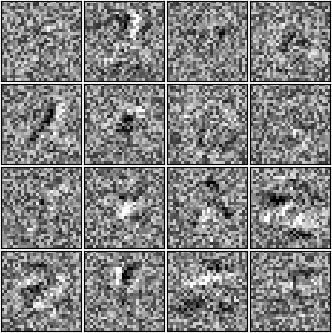
\includegraphics[width=0.5\textwidth]{img/MLP_Weights.png}
        \end{center}
      }
    \end{block}
  \end{textblock}
\end{frame}


%\section{A more convolved example: \acl{CNN}}


\begin{frame}
  \frametitle{\acl{CNN}: Introduction}

  \begin{textblock}{90}(5, 15)
    \begin{itemize}
    \item Introduced in 1989 - 1995
    \item Specialized for image-like structures
    \item Once again roughly biologically inspired
    \item Influential in the rise of deep-learning
    \item Same task than in the previous section
    \end{itemize}
  \end{textblock}
\end{frame}



% This frame allows to jump to frames explaining layers (file
% appendix_cnn)
\begin{frame}
  \note{
    \begin{itemize}
    \item Feed-forward
    \item Special layers
    \item Structure of images
    \end{itemize}
  }
  \frametitle{\acl{CNN}: Computation}
  \hypertarget<4>{CNN_Overview_Convolutional}{}
  \hypertarget<5>{CNN_Overview_Pooling}{}

  \begin{textblock}{90}(5,10)
    \begin{center}
      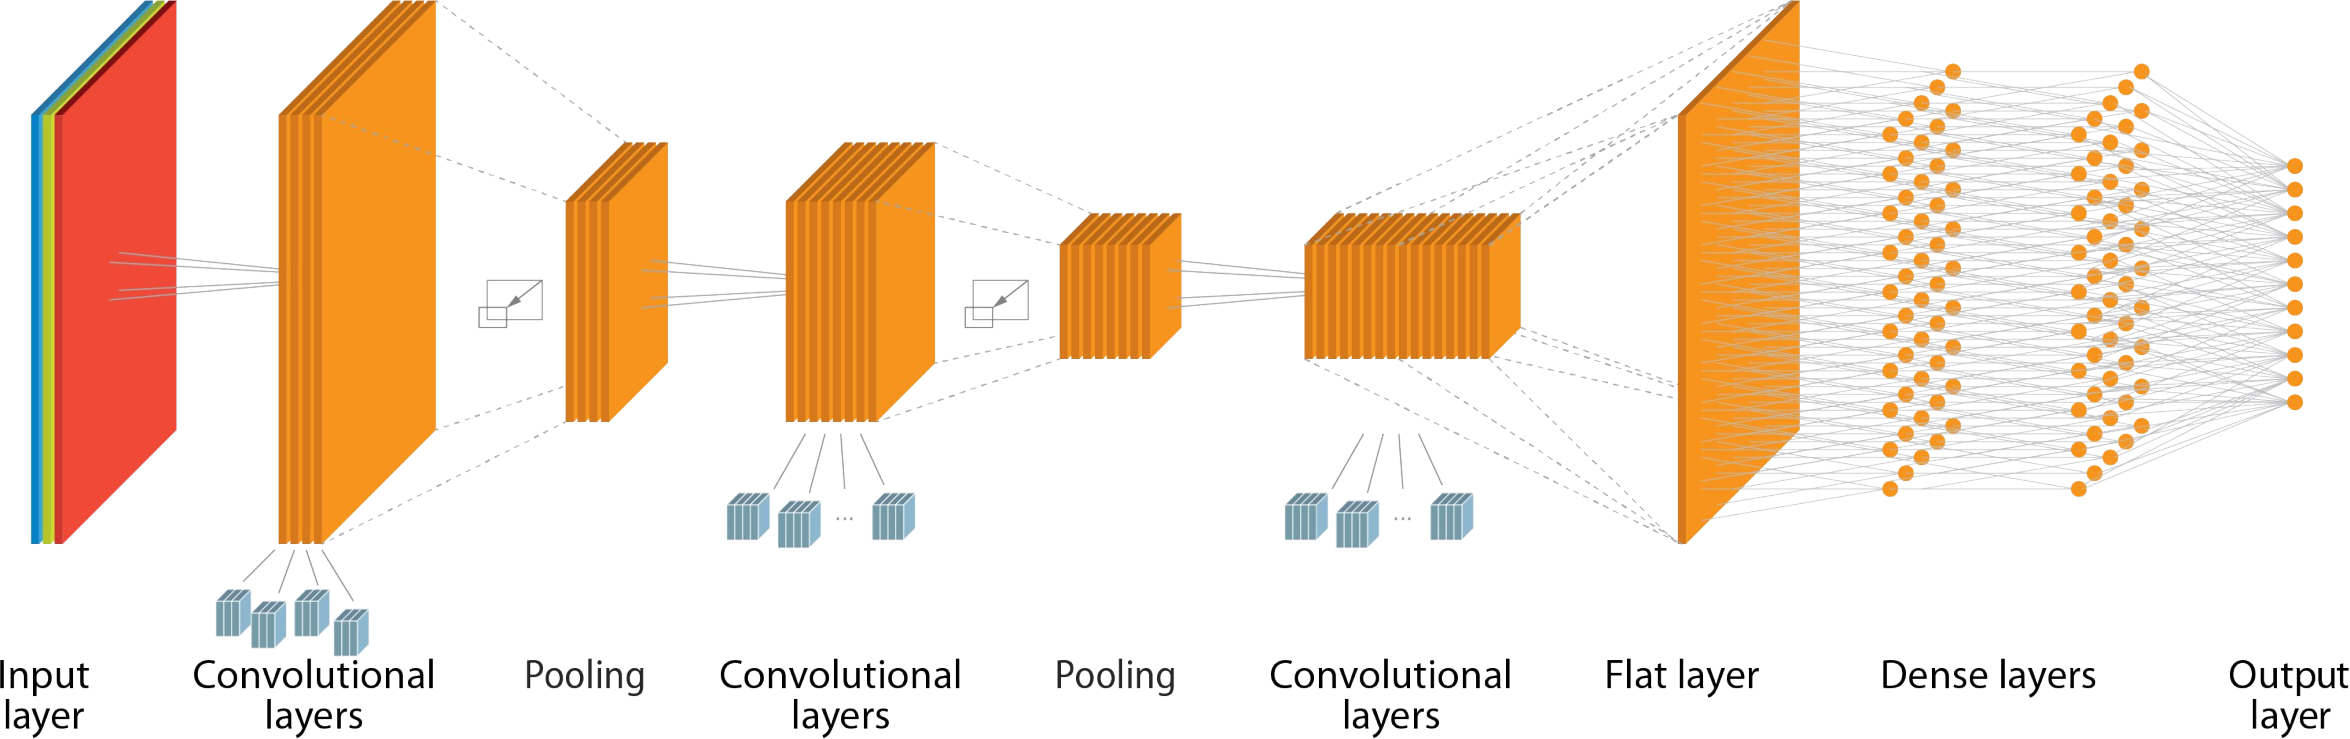
\includegraphics[width=\textwidth]{img/CNN.png}
      Taken from FIDLE
    \end{center}
  \end{textblock}

  \begin{textblock}{45}(5,57)
    \begin{itemize}
    \item Feed-forward architecture
    \item<2-> \ac{MLP} at the end
    \item<3-> Special hidden layers:
      \begin{itemize}
      \item Convolutional layers \hyperlink{Convolutional_Layers}{\beamerbutton{Details}}
        \onslide<4->{
          \begin{itemize}
          \item Kernels are learned
          \end{itemize}
        }
      \item Pooling layers \hyperlink{Pooling_Layers}{\beamerbutton{Details}}
        \onslide<5->{
          \begin{itemize}
          \item No learning
          \end{itemize}
        }
      \end{itemize}
    \end{itemize}
  \end{textblock}

  \begin{textblock}{45}(50,57)
    \onslide<6->{
      \begin{itemize}
      \item The idea is that the layers extract more and more abstract features
        (and then classify with the \ac{MLP}
      \item Weights are shared:
        \begin{itemize}
        \item Less parameters to learn
        \item Translation invariant features
        \end{itemize}
      \item Use the \emph{structure} of the image
      \item Many hyper-parameters
      \end{itemize}
    }
  \end{textblock}
\end{frame}


\begin{frame}
  \note{
    \begin{itemize}
    \item We can use back-propagation but we must do some computation
    \item Don't present the computation
    \end{itemize}
  }
  \frametitle{\acl{CNN}: Learning}

  \begin{textblock}{90}(5, 15)
    \begin{itemize}
    \item<1-> Same general principle: gradient descent of a loss function
    \item<2-> It's a feed-forward architecture so we know we can use back-propagation
    \item<3-> We have to compute the gradients for convolutional layers!
    \end{itemize}
  \end{textblock}

  \begin{textblock}{90}(5, 30)
    \onslide<4->{
      \begin{center}
        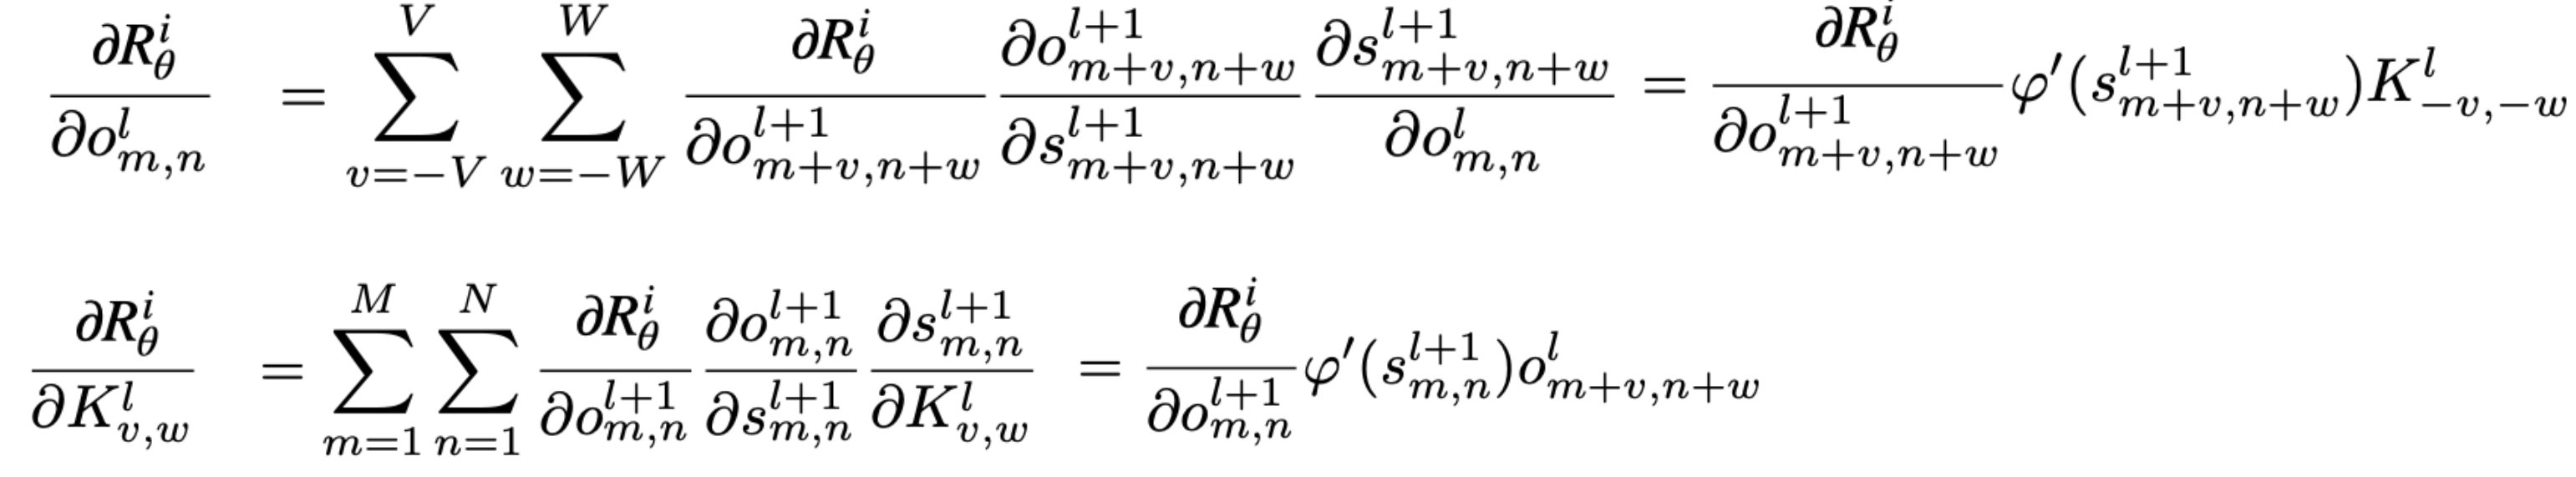
\includegraphics[width=\textwidth]{img/Backpropagation_CNN.png}
      \end{center}
      Taken from FIDLE (notations slightly different ($\varphi \leftrightarrow
      \activFunc$, $R \leftrightarrow \lossFunc$))
    }
  \end{textblock}
\end{frame}


\begin{frame}
  \note{
    \begin{itemize}
    \item Present results:
      \begin{itemize}
      \item 3 times less errors => 3 times less manual intervention when sorting
        letters
      \item Results IRL
      \end{itemize}
    \end{itemize}
  }
  \frametitle{\acl{CNN}: Results}

  \begin{textblock}{90}(5, 15)
    \begin{block}{Results}
      \begin{itemize}
      \item Error rate on MNIST test set $< 1\%$
      \item<2-> Competitive with other methods
      \item<3-> Integrated in some cheque reading systems in 1996
      \item<4-> Much better than \ac{MLP} for other tasks/datasets
      \end{itemize}
    \end{block}
  \end{textblock}

\end{frame}


\begin{frame}
  \note{
    \begin{itemize}
    \item Activation maps are image-like
    \end{itemize}
  }
  \frametitle{\acl{CNN}: Interpretation}

  \begin{textblock}{90}(5, 15)
    \begin{block}{Interpretation}
      \onslide<2->{
        Plot the activations:
        \begin{center}
          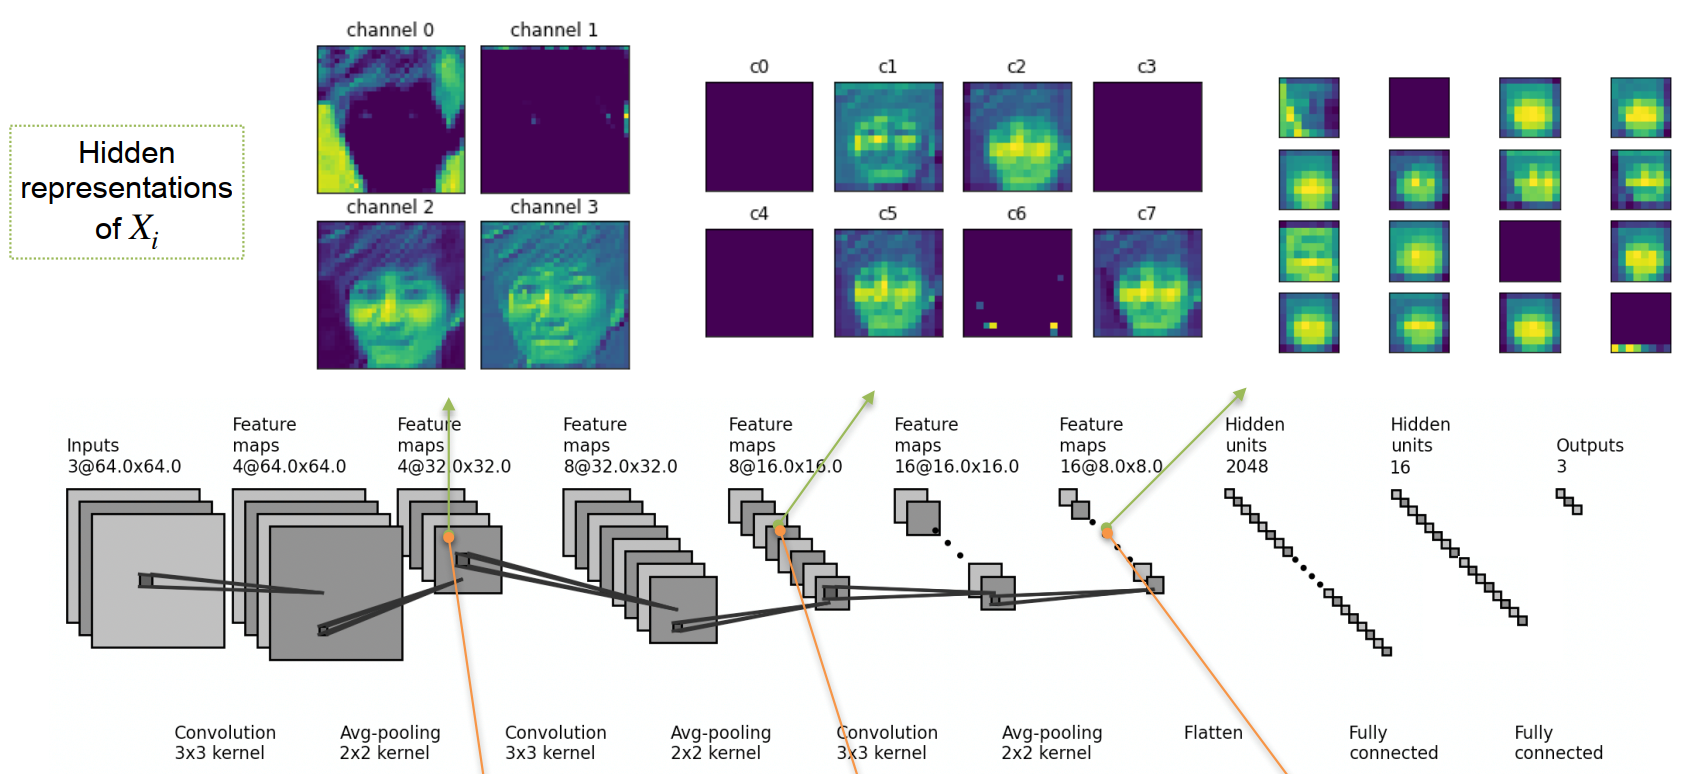
\includegraphics[width=\textwidth]{img/CNN_Interpretation.png}
        \end{center}
        First layers are easier to interpret
      }
      \end{block}
  \end{textblock}

\end{frame}


\begin{frame}
  \frametitle{What have we learned so far?}

  \begin{textblock}{90}(5, 15)
    \begin{itemize}
    \item<1-> No magic!
      \begin{itemize}
      \item To develop a new model, YOU have to do the maths
      \item YOU have to do the learning, tune the hyper-parameters, \etc{}
      \end{itemize}
    \item<2-> A bit of Neural Networks:
      \begin{itemize}
      \item Neurons: weighted sum and activation function
      \item Architecture: layers and weights
      \item Learning: back-propagation
      \end{itemize}
    \item<3-> Neural networks are very flexible:
      \begin{itemize}
      \item Mathematical foundations are not great, not terrible
      \item Be very careful with biological analogies
      \end{itemize}
    \item<4-> \ac{ML} is not only about models:
      \begin{itemize}
      \item Understand the type of data to design a model
      \item Need a lot of data \& computational power
      \item Data hell
      \item It's a job!
      \end{itemize}
    \end{itemize}
  \end{textblock}
\end{frame}


\section{Overview of \ac{ML}}

\subsection{Problems \& tasks}

\begin{frame}
  \note{
    \begin{itemize}
    \item Present classic supervised learning
    \end{itemize}
  }
  \frametitle{Supervised learning (1/2)}

  \begin{textblock}{90}(5,15)
    % Inspired by figure 3.4 in \cite{barra2021} (p. 82)
    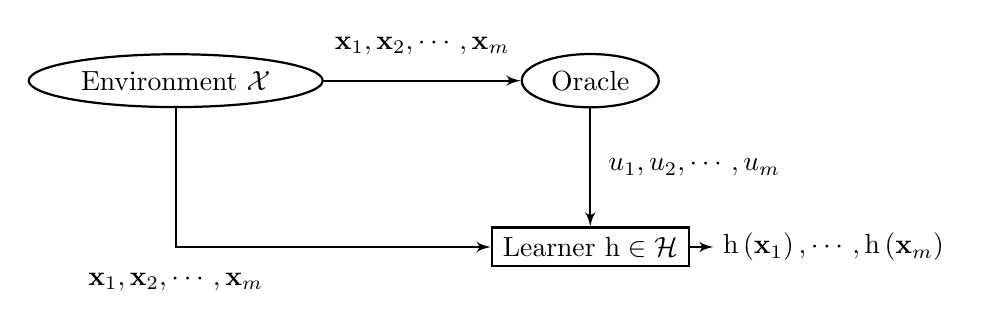
\begin{tikzpicture}
      \tikzstyle{line} = [draw, -latex', thick]
      \def\examples{$\example_1, \example_2, \cdots, \example_{\nTrainingSamples}$}
      \def\labels{$\knownLabel_1, \knownLabel_2, \cdots, \knownLabel_{\nTrainingSamples}$}
      \def\predictions{${\footnotesize\apply{\hyp}{\example_1}, \cdots, \apply{\hyp}{\example_{\nTrainingSamples}}}$}

      % Environment
      \def\env{Environment}
      \node[minimum width=2.5cm,ellipse,draw,thick] (\env) at (0, 0) {\env{} $\exampleSet$};

      % Oracle
      \def\oracle{Oracle}
      \node[ellipse,draw,thick,right = 2.5cm of \env] (\oracle) {\oracle{}};

      % Learner
      \def\learner{Learner}
      \node[minimum width=2.5cm,draw,thick,below = 1.5cm of \oracle] (\learner) {\learner{} $\hyp \in \hypSet$};

      % Output of learner
      \def\output{Output}
      \node[right = 0.3cm of \learner] (\output) {\predictions};

      % \env -> \oracle & \env -> \learner
      \path[line] (\env) -- node[above=0.2cm] {\examples} (\oracle);
      \path[line] (\env) -- +(0,-1) |- node[below=0.2cm] {\examples} (\learner);

      % \oracle -> learner
      \path[line] (\oracle) -- node[right=0.1cm] {\labels} (\learner);

      % \learner -> \output
      \draw[line] (\learner) -- (\output);
    \end{tikzpicture}
  \end{textblock}

  \begin{textblock}{90}(5,55)
    \begin{itemize}
    \item The environment generates $\nTrainingSamples$ examples
      $\drawFrom{\example}{\pdfExample}$ (unknown)
    \item The oracle labels them according to a function $\targetFunc: \exampleSet
      \mapsto \labelSet$ or a probability distribution $\condpdfLabelExample$ (unknown)
    \item The learner has a set of functions $\exampleSet
      \mapsto \labelSet$, noted $\hypSet$
    \item The goal is to find $\opt{\hyp} \in \hypSet$ that approximates
      $\targetFunc$
      \begin{itemize}
      \item Note that it's possible that $\targetFunc \not\in \hypSet$
      \end{itemize}
    \end{itemize}
  \end{textblock}
\end{frame}


\begin{frame}
  \note{
    \begin{itemize}
    \item Give some details about the tasks
    \item Link to statistics
    \end{itemize}
  }
  \frametitle{Supervised learning (2/2)}

  \begin{textblock}{90}(5, 15)
    \begin{block}{Tasks in supervised learning}
      \begin{itemize}
      \item Classification: $\labelSet = \setext{1,..,\nClasses}$
        \begin{itemize}
        \item Binary classification (concept learning): $\card{\labelSet} = 2$
        \item Multi-class classification
        % \item Examples: classify an animal into a species
        \end{itemize}
      \item Multi-label classification (multi-output classification): one input can have
        several classes (potentially a variable number)
        \begin{itemize}
        \item Examples: tagging text or images
        \end{itemize}
      \item Regression: $\labelSet \subset \setR^n$
      \item Ranking
      \end{itemize}
    \end{block}
  \end{textblock}
\end{frame}


\begin{frame}
  \note{
    \begin{itemize}
    \item Present unsupervised learning \& link to statistics
    \end{itemize}
  }
  \frametitle{Unsupervised learning}

  \begin{textblock}{90}(5,15)
    % Inspired by figure 3.4 in \cite{barra2021} (p. 82)
    \begin{tikzpicture}
      \tikzstyle{line} = [draw, -latex', thick]
      \def\examples{$\example_1, \example_2, \cdots, \example_{\nTrainingSamples}$}
      \def\labels{$\knownLabel_1, \knownLabel_2, \cdots, \knownLabel_{\nTrainingSamples}$}
      \def\predictions{${\footnotesize\apply{\hyp_{\params}}{\example_1}, \cdots, \apply{\hyp_{\params}}{\example_{\nTrainingSamples}}}$}

      % Environment
      \def\env{Environment}
      \node[minimum width=2.5cm,ellipse,draw,thick] (\env) at (0, 0) {\env{} $\exampleSet$};

      % Oracle is hidden but we need it for node position
      \invisible{
        \def\oracle{Oracle}
        \node[ellipse,draw,thick,right = 2.5cm of \env] (\oracle) {\oracle{}};
      }

      % Learner
      \def\learner{Learner}
      \node[minimum width=2.5cm,draw,thick,below = 1.5cm of \oracle] (\learner) {\learner{} $\hyp_{\params} \in \hypSet$};

      % Output of learner
      \def\output{Output}
      \node[right = 0.3cm of \learner] (\output) {\predictions};

      % \env -> \learner
      \path[line] (\env) -- +(0,-1) |- node[below=0.2cm] {\examples} (\learner);

      % \learner -> \output
      \draw[line] (\learner) -- (\output);
    \end{tikzpicture}
  \end{textblock}

  \begin{textblock}{90}(5,55)
    \begin{itemize}
    \item The environment generates $\nTrainingSamples$ examples
      $\drawFrom{\example}{\pdfExample}$ (unknown)
    \item No oracle
    \item The learner tries to model the environment:
      \begin{itemize}
      \item Clustering: find groups in $\exampleSet$
      \item Density estimation: find $\pdfExample$
      \end{itemize}
    \end{itemize}
  \end{textblock}
\end{frame}


\begin{frame}{Learning protocol}
  \note{
    \begin{itemize}
    \item Briefly present the notion of learning protocol
    \item Difference with statistics
    \end{itemize}
  }

  \begin{textblock}{90}(5,15)
    \begin{block}{}
      The learning protocol describes the interaction between the learner and the
      environment:
      \begin{itemize}
      \item<2-> Batch learning: all $\nTrainingSamples$ examples are given
      \item<3-> Online learning: examples are given one by one and the learner
        tries to improve on each
      \item<4-> More complex protocols:
        \begin{itemize}
        \item Active learning: the learner searches for examples
        \end{itemize}
      \end{itemize}
    \end{block}
  \end{textblock}
\end{frame}


\begin{frame}{Other levels of supervision}
  \note{
    \begin{itemize}
    \item
    \end{itemize}
  }

  \begin{textblock}{90}(5, 15)
    You can imagine other levels of supervision:
    \begin{itemize}
    \item<2-> Semi-supervised: you have $\ell$ labelled examples and
      $\nTrainingSamples - \ell$ unlabelled examples
      \begin{itemize}
      \item Can you use the unlabelled examples to improve the classification?
      \end{itemize}
    \item<3-> Self-supervised: learn a representation of unlabelled data that is
      useful for later supervised learning
    \item<4-> Reinforcement learning: the learner receive delayed and sparse signal
      from the oracle about his performance:
    \item<5-> .. and mix them
      \begin{itemize}
      \item ChatGPT is trained in 3 phases: first in a self-supervised phase
        (predict the next sentence in a phrase),
        then in a supervised phase (predicting requests) and first and then with
        reinforcement learning (to avoid some behaviour)
      \end{itemize}
    \end{itemize}
  \end{textblock}

  \begin{textblock}{90}(5, 85)
    \onslide<6->{
      The difference between the task, the protocol or the technique
      is not always clear
    }
  \end{textblock}
\end{frame}


\begin{frame}
  \frametitle{How to approximate $\targetFunc$? (1/2)}

  \begin{textblock}{90}(5, 10)
    \begin{block}{True risk}
      Suppose that we have a loss function $\lossFunc: \exampleSet \times \labelSet \mapsto
      \setR^+$ that evaluates how bad one example is predicted by an hypothesis $\hyp$.
      The true risk of $\hyp$ is then:
      \begin{equation*}
        \begin{split}
          \apply{\risk}{\hyp} & = \expectation{\apply{\lossFunc}{\apply{\hyp}{\example}, \predLabel}}\\
                              & = \int_{\example \in \exampleSet, \predLabel \in \exampleSet}
          \apply{\lossFunc}{\apply{\hyp}{\example}, \predLabel} \pdfExampleLabel \intover{\example} \intover{\predLabel}
        \end{split}
      \end{equation*}
    \end{block}
\end{textblock}

  \begin{textblock}{90}(5, 45)
    \begin{block}{Examples of loss functions}
      \begin{itemize}
      \item For classification:
        \begin{itemize}
        \item 0-1 loss:
          $\apply{\lossFunc}{\apply{\hyp}{\example}, \predLabel} =
          \begin{cases}
            0 & \text{if $\apply{\hyp}{\example} \ne \predLabel$} \\
            1 & \text{if $\apply{\hyp}{\example}  =  \predLabel$}
          \end{cases}
          $
        \item Logistic loss (binary probabilistic classification): $\apply{\lossFunc}{\apply{\hyp}{\example},
            \predLabel} =
          -\apply{\log}{\frac{\apply{\hyp}{\example}}{1-\apply{\hyp}{\example}}}$
        \item Non-symmetric loss function
        \end{itemize}
      \item For regression:
        \begin{itemize}
        \item Quadratic: $\apply{\lossFunc}{\apply{\hyp}{\example}, \predLabel}
          = \left( \apply{\hyp}{\example} - \predLabel \right)^2$
        \end{itemize}
      \end{itemize}
    \end{block}
  \end{textblock}
\end{frame}


\begin{frame}
  \frametitle{How to approximate $\targetFunc$? (2/2)}

  \begin{textblock}{90}(5, 10)
    \begin{block}{Optimal hypothesis}
      The best hypothesis $\opt{\hyp}$ is:
      \[
        \opt{\hyp} = \argmin_{\hyp \in \hypSet} \apply{\risk}{\hyp}
      \]
    \end{block}
  \end{textblock}

  \begin{textblock}{90}(5, 35)
    \begin{block}{Generative \vs{} Discriminative approach}
      \begin{itemize}
      \item Generative learning
      \item Discriminative learning
      \end{itemize}
    \end{block}
  \end{textblock}
\end{frame}


\subsection{Theoretical approaches of supervised learning}

\begin{frame}
  \frametitle{Introduction}

  \begin{textblock}{100}(5,10)
    \begin{itemize}
    \item Several approaches have been developped to understand
      supervised learning
    \item Much less for other cases
    \end{itemize}
  \end{textblock}
\end{frame}




\section{Deep Learning}

\begin{frame}{Project Data to solve complex tasks}
    \note{Deep learning relies on several key principles that enable it to effectively learn from complex data}
  

    \begin{center}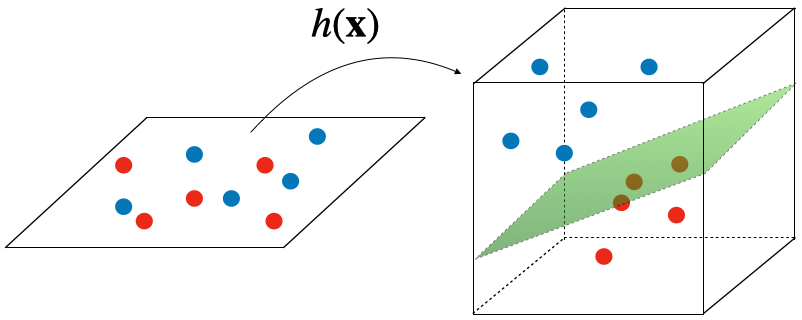
\includegraphics[width=200px]{img/projection.png}\end{center}
    \vspace{0.5cm}
    \begin{itemize}
        \note{Consequence of Cover's theorem (computational learning theory): set of training data that is not linearly separable, can with high probability be transformed into a training set that is linearly separable by projecting it into a higher-dimensional space via some non-linear transformation}
        \item A complex pattern-classification problem, cast in a high-dimensional space nonlinearly, is more likely to be linearly separable than in a low-dimensional space, provided that the space is not densely populated (Cover's theorem).
        \item Primary theoretical motivations for the use of non-linear kernel methods in ML (Poynomial and Radial Basis Function kernels in SVM)
    \end{itemize}
  
  
  \end{frame}

  \begin{frame}{Deep Learning}  

    \begin{textblock}{40}(65, 20)
        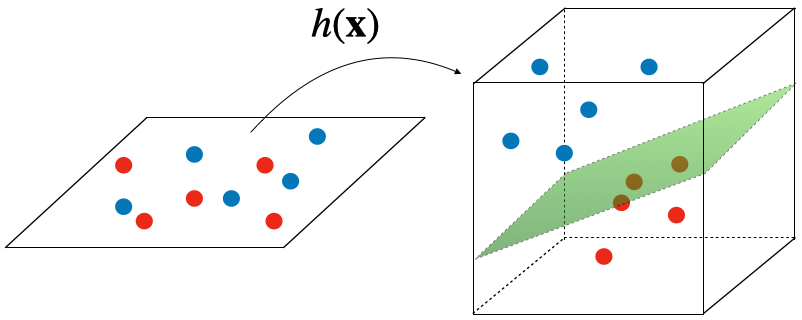
\includegraphics[width=110px]{img/projection.png}
    \end{textblock}
    \begin{textblock}{40}(65, 40)
      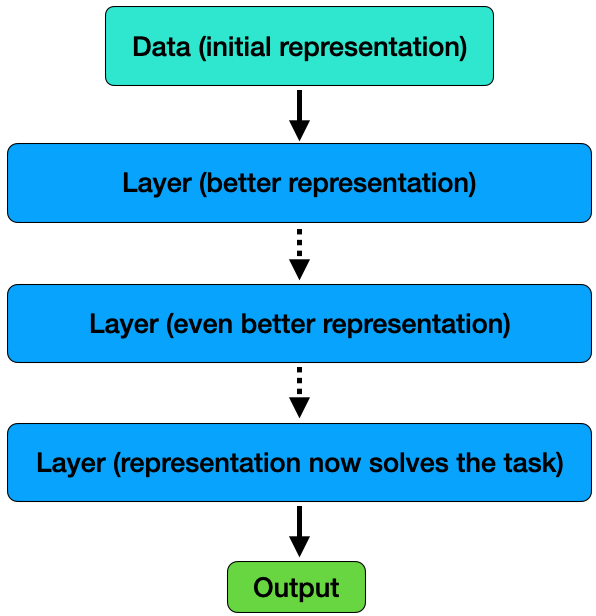
\includegraphics[width=120px]{img/projection_dl.png}
    \end{textblock}

    
    \begin{textblock}{60}(1, 15)
        \begin{itemize}
            \item Deep learning is the subset of machine learning methods based on Neural Networks (NN)
            \item NN model learns a complex non-linear function that will project the data in a high-dimension space where the data are linearly separable or where we have a better representation of the data to solves the task
            \item To do so, NN model project the data non-linearly successively through several neural layers improving representation at each step
            \item The adjective "deep" refers to the use of multiple layers in the network
          \end{itemize}
    \end{textblock}
  
  
  \end{frame}

\begin{frame}{Deep Learning}
  \begin{textblock}{60}(1, 15)
    \begin{itemize}
      \item These layers performs operations which either:
      \begin{itemize}
        \item Project non-linearly (typically linear-layer + non linear activation function)
        \item Capture the structural patterns and relationships within the data (Convolutional layers in Convolutional Neural Network (CNN), Attention mechanisms in Transformers, Aggregation functions in Graph Neural Network (GNN))
      \end{itemize}
      \item The combination of non-linear projections and the capture of structural patterns allows neural network models to learn complex non-linear functions, projecting data into a space where their representations can solve the task effectively
      \item Two examples: The transformers and the GNNs
    \end{itemize}
  \end{textblock}

  \begin{textblock}{40}(65, 20)
    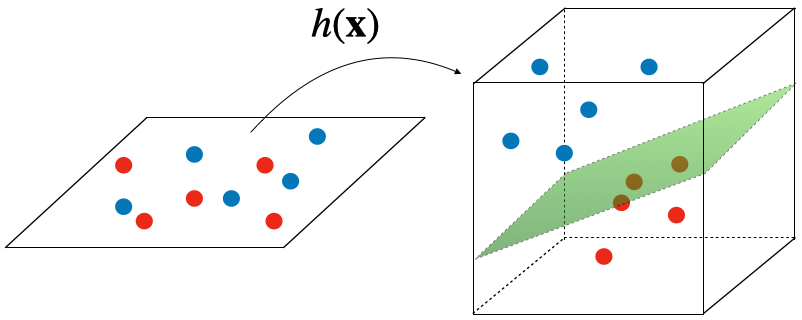
\includegraphics[width=110px]{img/projection.png}
  \end{textblock}
  \begin{textblock}{40}(65, 40)
    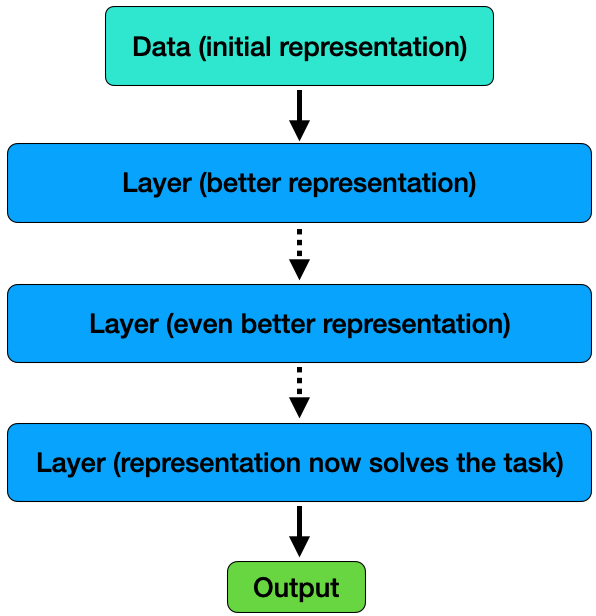
\includegraphics[width=120px]{img/projection_dl.png}
  \end{textblock}

\end{frame}


%\subsection{A few example}

\begin{frame}{Transformers: Attention Mechanisms}
  \begin{itemize}
      \item Something often heard: Large Language Models (LLMs) predict "only" the next word in a sentence, the most likely word.
      \item That's true. But the real question is how do LLMs do it??
      \item To answer this question, we need to understand the architectures on which they are based: Transformers and their core mechanism: the attention mechanism
  \end{itemize}
\end{frame}


\begin{frame}{Transformers: Attention Mechanisms}
    \begin{itemize}
        \item Transformers are a type of model architecture primarily used in the field of natural language processing (NLP)
        \item They have become foundational for tasks such as translation, text generation, text summarization, and sentiment analysis
        \item Introduced in the seminal paper "Attention is All You Need" in 2017, transformers represent a significant shift from previous Recurrent Neural Network models approachs in NLP
      \end{itemize}
\end{frame}

\begin{frame}{Transformers: Attention Mechanisms}
    \begin{textblock}{50}(2, 15)
        Goal: identify and attend to most important features in input that are relevant to the semantic meaning
    \end{textblock}
    \begin{textblock}{48}(2, 35)
        \setbeamercovered{transparent}

        \onslide<1->{1. Input \textbf{embeddings}}

        \onslide<2->{2. Encode \textbf{position} information}

        \onslide<3->{3. Compute 3 independant linear projection: \textbf{query, key, value}}

        \onslide<6->{4. Compute \textbf{attention weighting}}   
        
        \onslide<10->{5. Ponderate value features with \textbf{attention scores}}

        %\onslide<11->{These operations form a self attention head.}

        %\onslide<11->{Multi head attention : Multiple head attend on different type of complex relationship in the input sequence.}


    \end{textblock}
      \note{
        \begin{itemize}
          \item the firts step is to encode the sequence in a embeddings space (in which the words close semanticall are close in the space) and also encode postional encodings
          \item the next step is to take this encodings and figure out where to attend
          \item we compute Q, K, V withe separate neural network layers with separate set of weights that transform the encoding in a different way
          \item Now with this three matric the query the key the value we can compare them to each other to try to figure out where in that self-input the network should attend to what is important 
          \item And that's the key idea behind this similiraty metric or what you can think of an attention score
          \item Mathematically the way we can compare this two vectors to understand how similar they are is by taking the dot product. Capture how similar this vector,rather or not tey are pont ing in the same direction   
        \end{itemize}    
    }
    

    \begin{textblock}{48}(52, 25)
        \includegraphics<1>[width=150px]{img/transformer_1.png}
        \includegraphics<2>[width=150px]{img/transformer_2.png}
        \includegraphics<3>[width=150px]{img/transformer_3.png}
        \includegraphics<4>[width=150px]{img/transformer_4.png}
        \includegraphics<5>[width=150px]{img/transformer_5.png}
        \only<6-9>{Attention score: compute pairwise similarity between each query and key}
        \only<6-7>{How compute similarity between vectors of features?}
        \includegraphics<7>[width=150px]{img/transformer_6.png}
        \includegraphics<8>[width=150px]{img/transformer_7.png}
        \includegraphics<9>[width=150px]{img/transformer_8.png}
        \includegraphics<10>[width=150px]{img/transformer_9.png}
    \end{textblock}

\end{frame}

\begin{frame}{Transformers: Self and Multi-Head Attention}
  \begin{textblock}{60}(2, 15)
    \textbf{Scaled Dot-Product Attention} : \\  
    
    \[
    \text{Attention}(Q, K, V) = \text{softmax}\left(\frac{QK^T}{\sqrt{d_k}}\right)V
    \]

    These operations form a self-attention head that can plug into a larger network.\\ 
  \end{textblock}
  \begin{textblock}{60}(2, 52)
    \textbf{Multi-Head Attention} : \\
    We can multiply the attention head to enhance the model's ability by allowing it to capture different type of relationship between the element of the sequence
    \[
    \text{MultiHead}(Q, K, V) = \text{Concat}(\text{head}_1, \ldots, \text{head}_h)W^O
    \]
    where $\text{head}_i = \text{Attention}(QW_i^Q, KW_i^K, VW_i^V)$
  \end{textblock}

  \begin{textblock}{38}(62, 15)
    \begin{center}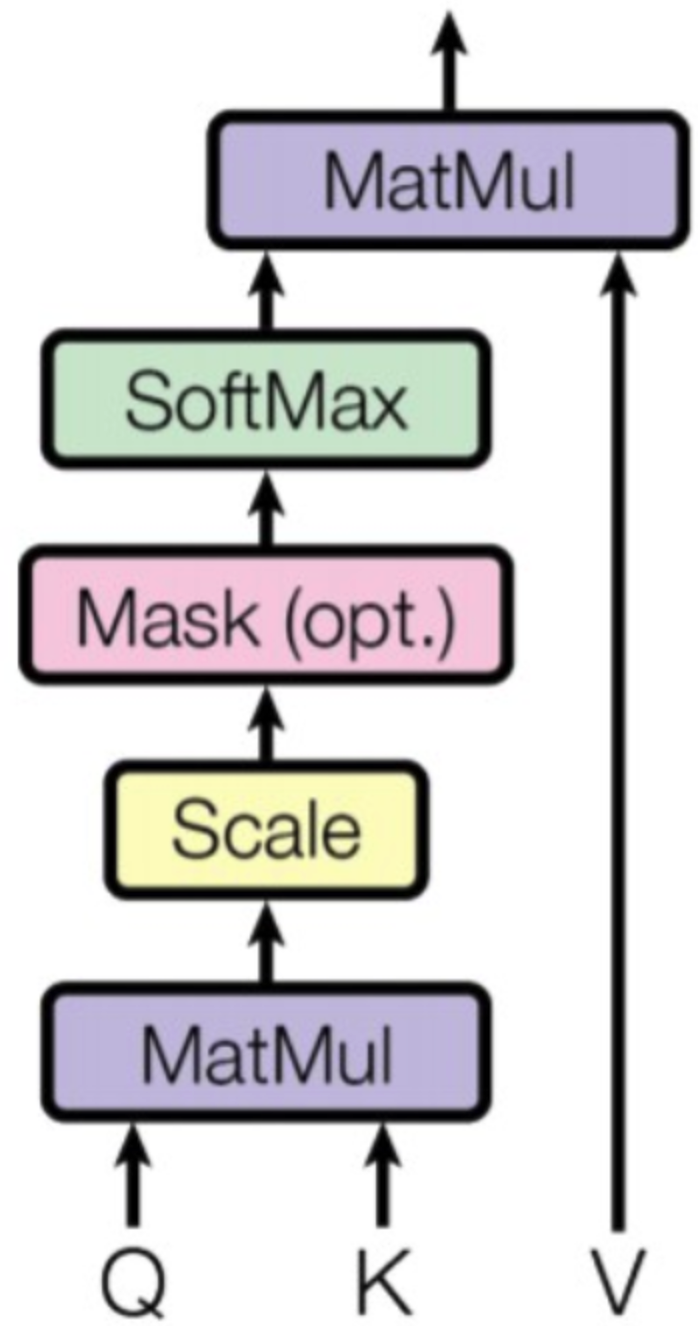
\includegraphics[width=40px]{img/transformer_10.png}\end{center}
    \begin{center}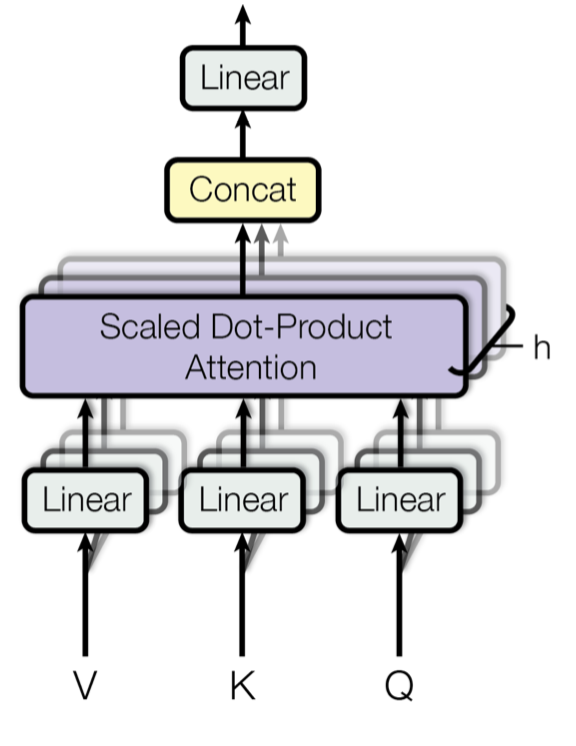
\includegraphics[width=80px]{img/transformer_11.png}\end{center}
  \end{textblock}

\end{frame}



\begin{frame}{Transformers in LLMs}
  \begin{textblock}{52}(4, 15)
    Transformers are essential in large language models (LLMs) due to their ability to process text sequences in a parallel and efficient manner

    \begin{itemize}
        \item \textbf{Encoding-Decoding} : Transformers use encoding layers to understand the context and decoding layers to generate text
        \item \textbf{Representation Learning} : LLMs learn rich representations of text by capturing long-term contextual relationship
    \end{itemize}

    \textbf{Transformer Architecture} : \\
    \begin{itemize}
        \item \textbf{Encoder} : Consists of multiple layers of attention and feed-forward networks
        \item \textbf{Decoder} : Similar to the encoder but with additional mechanisms for attention over the encoded input
    \end{itemize}
  \end{textblock}
  \begin{textblock}{35}(56, 28)
    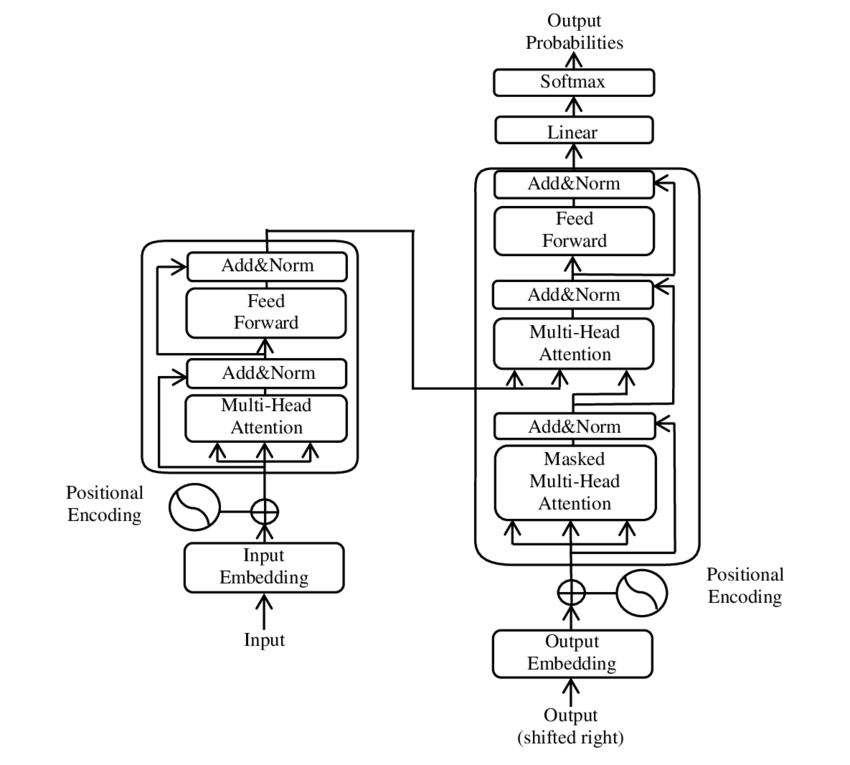
\includegraphics[width=170px]{img/transformer_architecture.png} % Make sure you have the image in the same folder or adjust the path.
  \end{textblock}
\end{frame}

\begin{frame}
  \frametitle{Transformers: other applications}
  \begin{itemize}
    \item Transformers have significantly impacted various fields beyond just NLP (image recognition, image generation, healthcare, autonomous vehicle, bioinformatics, etc)
    \item \textbf{AlphaFold 2 (Deepmind, 2021)}
  \end{itemize}

  \note{
    AlphaFold 2 is a groundbreaking artificial intelligence model developed by DeepMind that predicts the three-dimensional structures of proteins with remarkable accuracy.

    - Input and Data: amino acid sequence of a protein.  all the necessary information to determine the protein's structure
     multiple sequence alignments, to identify patterns and evolutionary information.

    - Attention Mechanism: The core of AlphaFold 2 is built on a deep learning architecture that employs an attention mechanism, similar to those used in language processing models like GPT-3. 
    
    This mechanism allows AlphaFold 2 to focus on specific parts of the protein sequence that are crucial for determining how the protein folds.

  }

  \begin{center}
    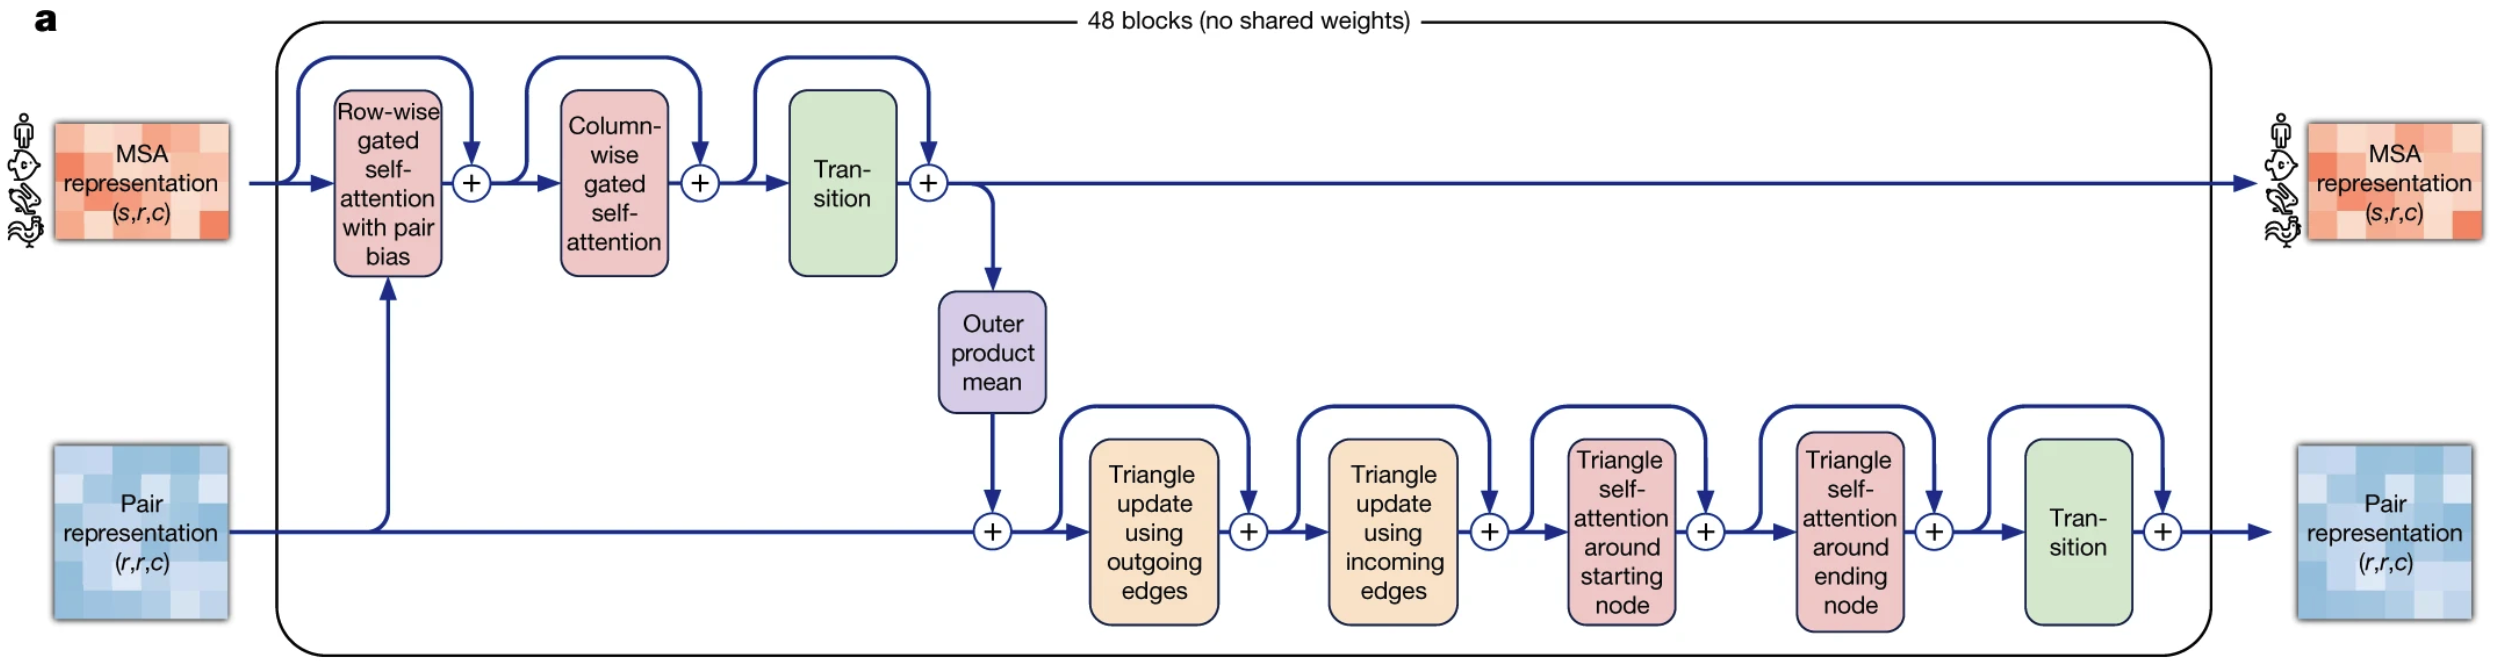
\includegraphics[width=200px]{img/alpha_fold_1.png}
    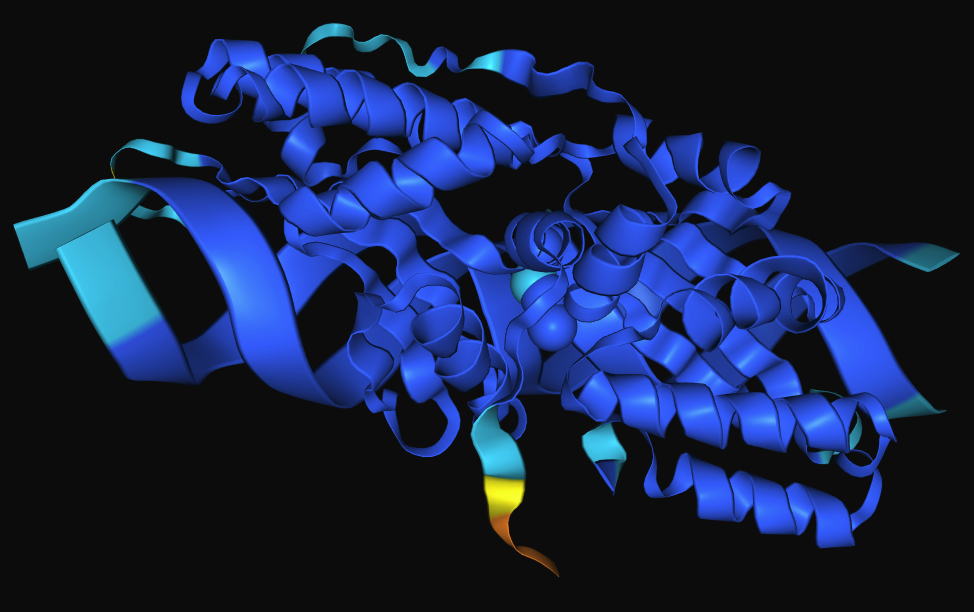
\includegraphics[width=110px]{img/alpha_fold_2.png}
  \end{center}
  

\end{frame}

\begin{frame}{Graph Neural Networks (GNNs)}
  \textbf{Geometric Deep Learning} \note{involves the study and development of deep learning models that can operate on non-Euclidean data such as graphs, manifolds, and other complex geometric structures}

  \begin{itemize}
      \item \textbf{Traditional Deep Learning} typically operates on Euclidean data (e.g., images, text)
      \item \textbf{Geometric Data} includes graphs, point clouds, and manifolds, which are not naturally represented in Euclidean space
  \end{itemize}

  \textbf{Graph Neural Networks} (GNNs) are a class of NN designed to perform inference on data described as \textbf{Graphs}: \note{They are particularly useful for tasks where the data is naturally represented as a graph structure.}
  \begin{itemize}
    \item \textbf{Nodes}: Represent entities in the graph.
    \item \textbf{Edges}: Represent relationships or interactions between entities
  \end{itemize}

\end{frame}

\begin{frame}{Graph Neural Networks (GNNs): Message Passing}

  \note{
    \textbf{Key Components of GNNs}:
    \begin{itemize}
        \item \textbf{Node Embeddings}: Each node is represented by a feature vector
        \item \textbf{Aggregation}: Combining information from neighboring nodes
        \item \textbf{Update}: Non-linearly project aggregation to compute new node embeddings
        \item \textbf{Message Passing}: Nodes exchange information with their neighbors to update their embeddings
        \item Message passing is repeated throuh all the GNN layers and allows the model to capture deep structural patterns in the graph 
      \end{itemize}
  }
    \begin{center}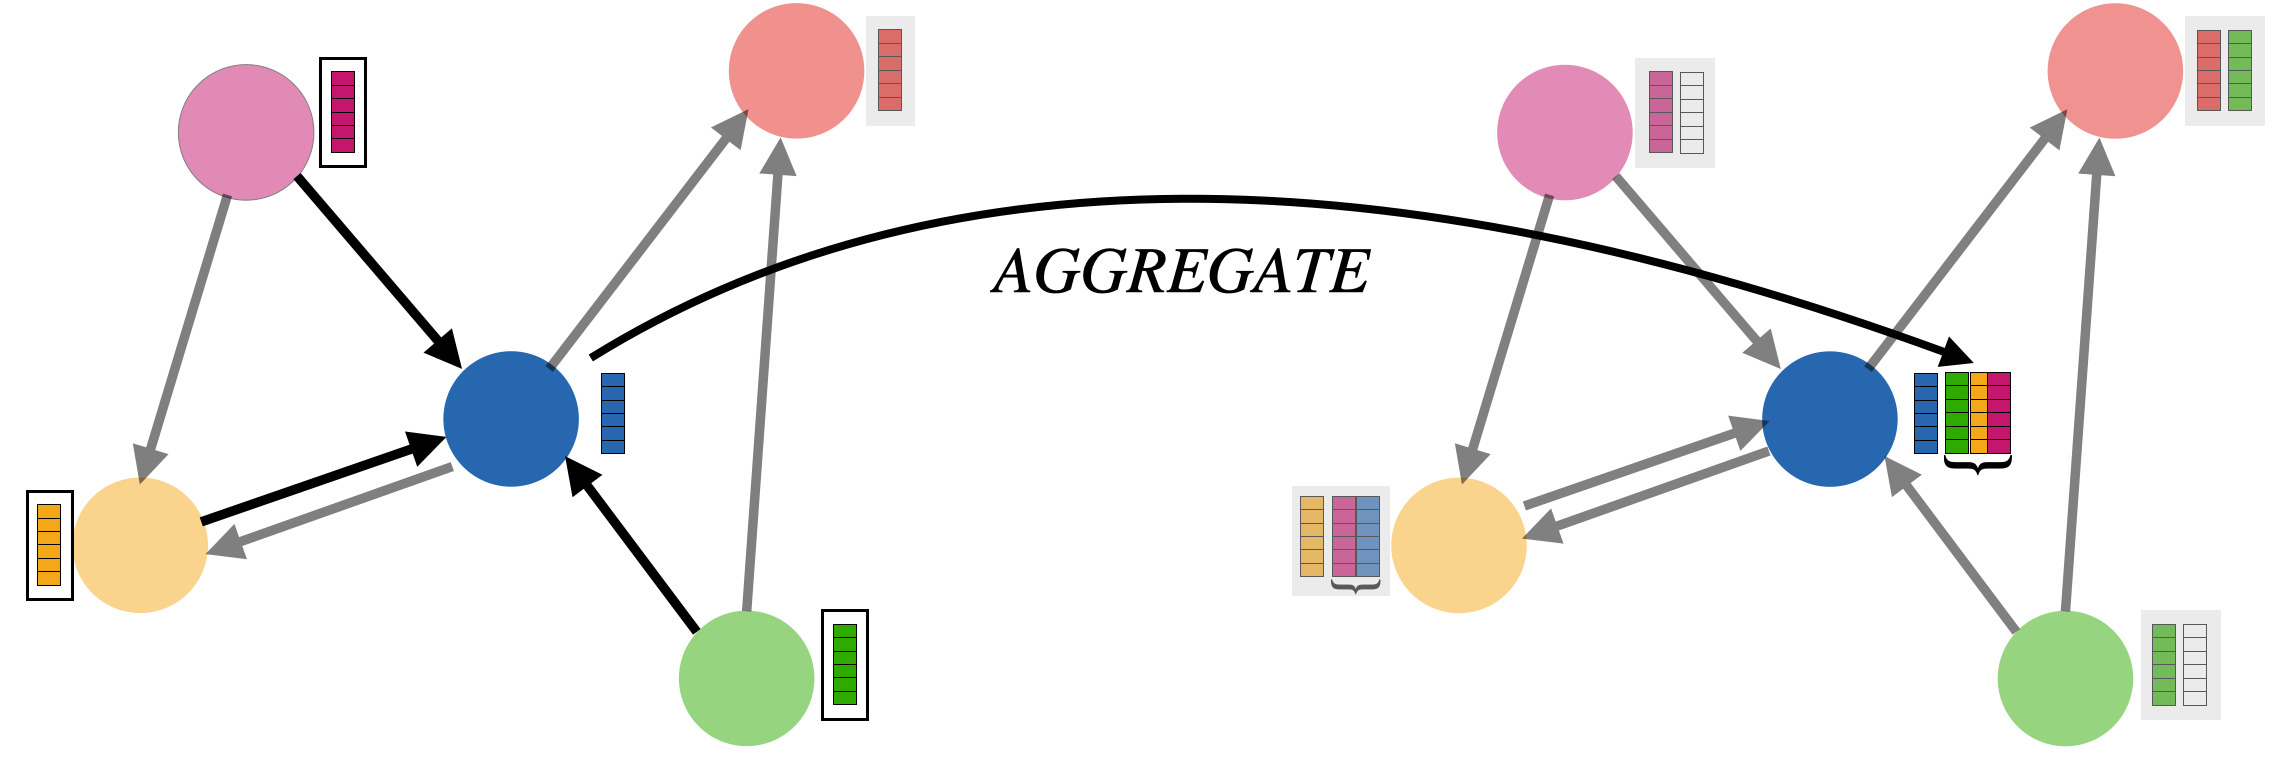
\includegraphics[width=200px]{img/gnn_aggregate.png}\end{center}
    \begin{center}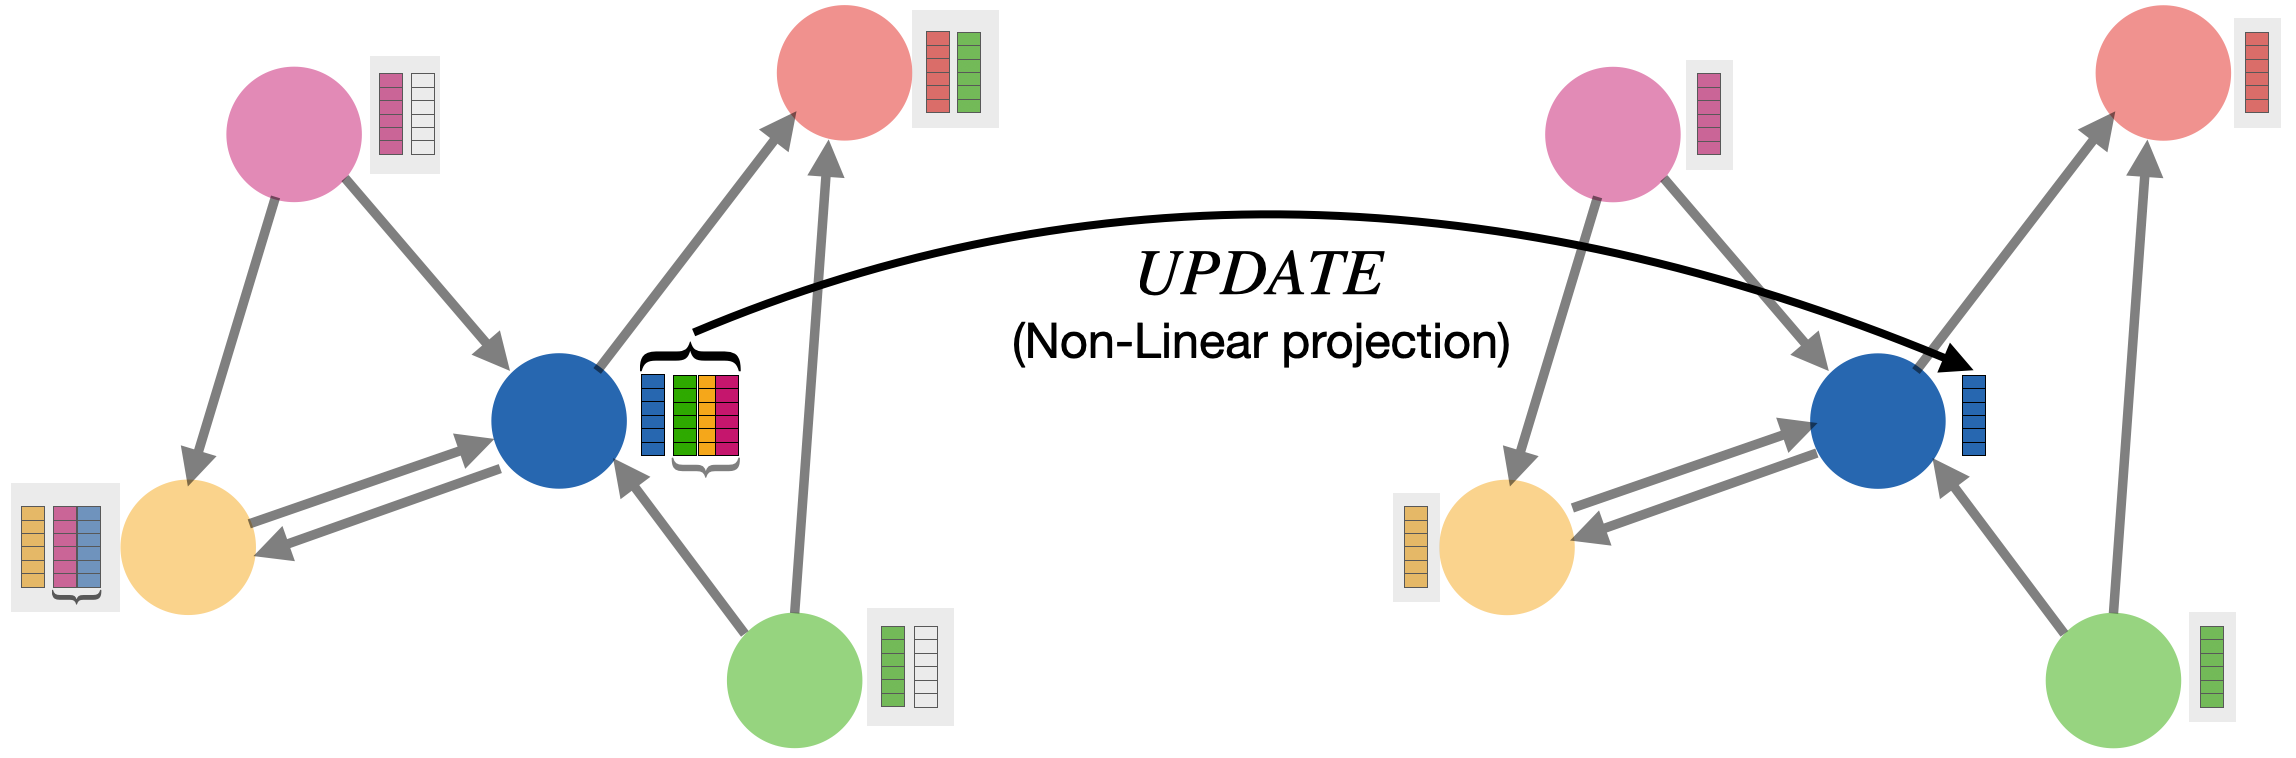
\includegraphics[width=200px]{img/gnn_update.png}\end{center}
  
  \textbf{Message Passing Formula}:
  \[
  h_i^{(k)} = \text{UPDATE}^{(k)}\left(h_i^{(k-1)}, \text{AGGREGATE}^{(k)}\left(\{h_j^{(k-1)} : j \in \mathcal{N}(i)\}\right)\right)
  \]
  where \(h_i^{(k)}\) is the embedding of node \(i\) at iteration \(k\), and \(\mathcal{N}(i)\) denotes the neighbors of node \(i\).

    \note{GNN can also be seenn as a generalization of convolution networks (Image seen as graphs) and transformers (sequence of text as a fully connected graph). They have a very powerfull expressiveness.}

\end{frame}

\begin{frame}
    \frametitle{Graph Neural Networks: applications}
    \begin{textblock}{90}(5, 15)
      \begin{itemize}
        \item Geometric deep learning is a booming topic in AI 
        \item Social Network analysis, Biological and Chemical Networks, Particle Physic, etc
        \item Widely used at LHC, GNNs especially suitable for sparse data of the detectors

      \end{itemize}
    \end{textblock}

    \begin{textblock}{40}(15, 45)
      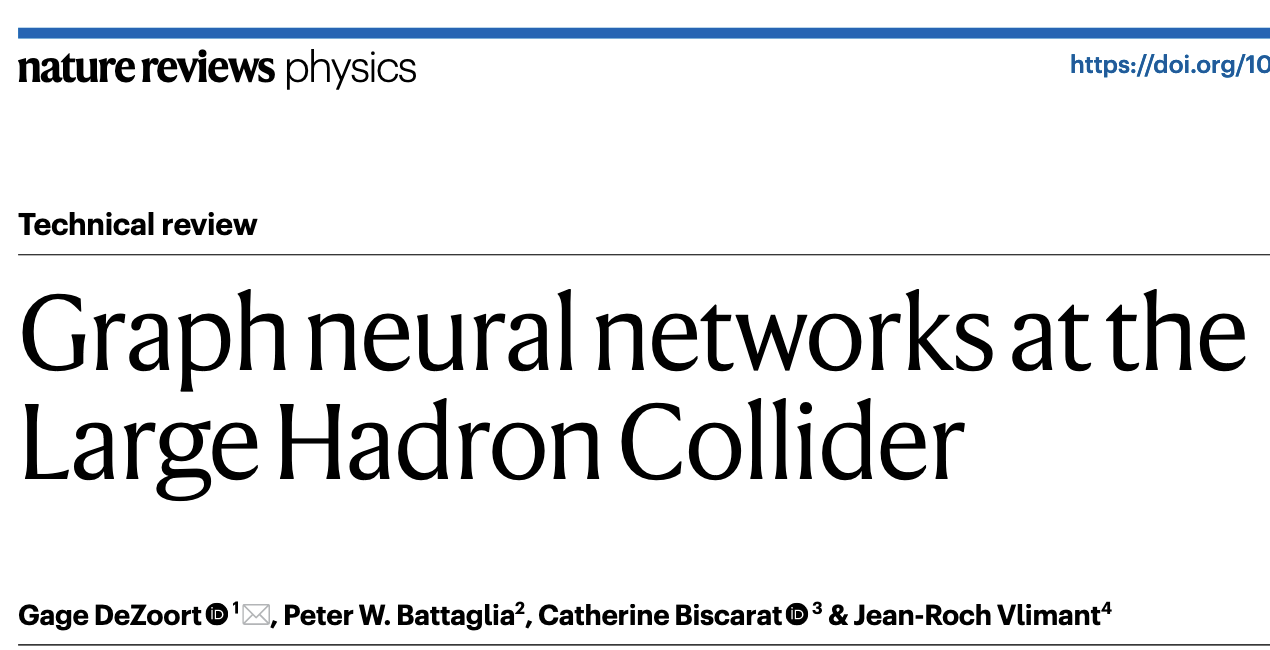
\includegraphics[width=140px]{img/gnn_lhc.png}
    \end{textblock}
    
    \begin{textblock}{30}(55, 40)
      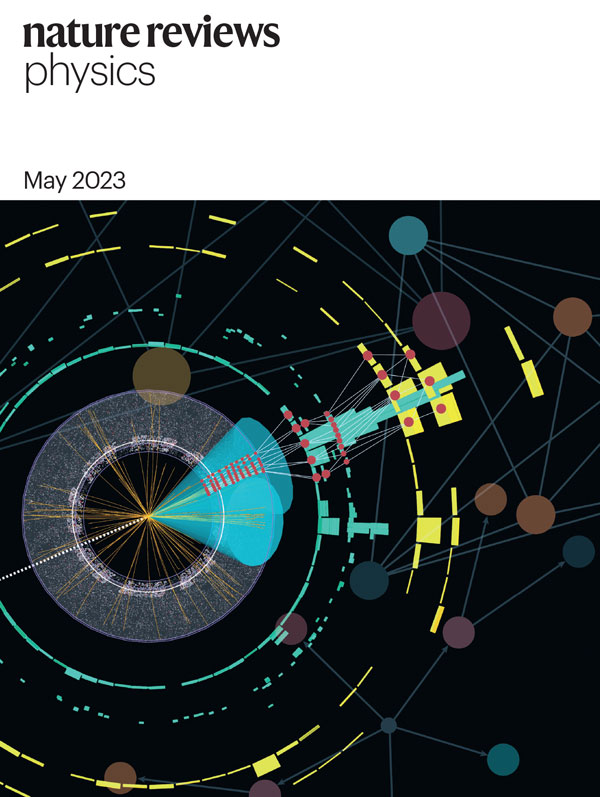
\includegraphics[width=110px]{img/gnn_lhc2.jpg}
    \end{textblock}

\end{frame}

%\subsection{New questions}

\begin{frame}
  \frametitle{GNN: an other interesting application example}
  \begin{textblock}{40}(2, 10)
    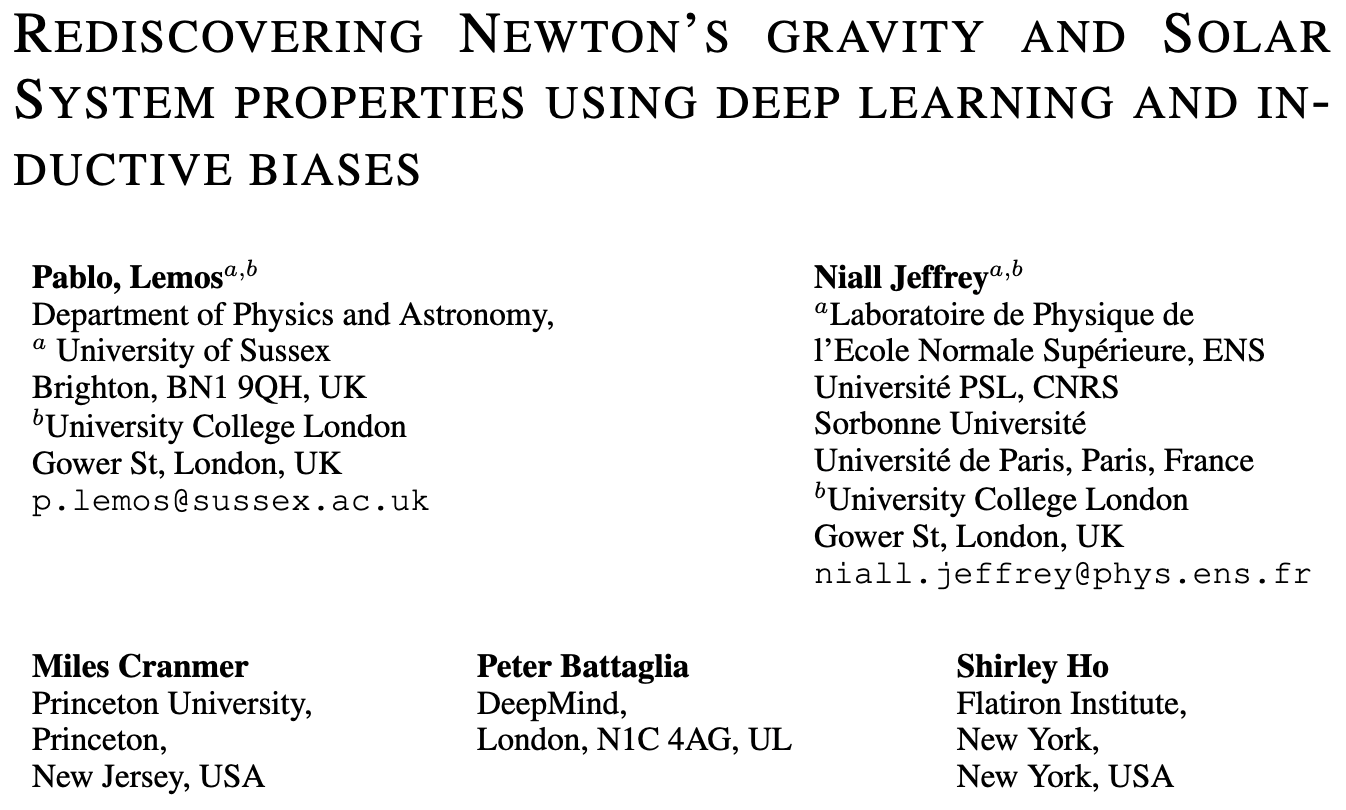
\includegraphics[width=150px]{img/retrieve_gravitation_laws_1.png}
  \end{textblock}
  \begin{textblock}{56}(44, 25)
    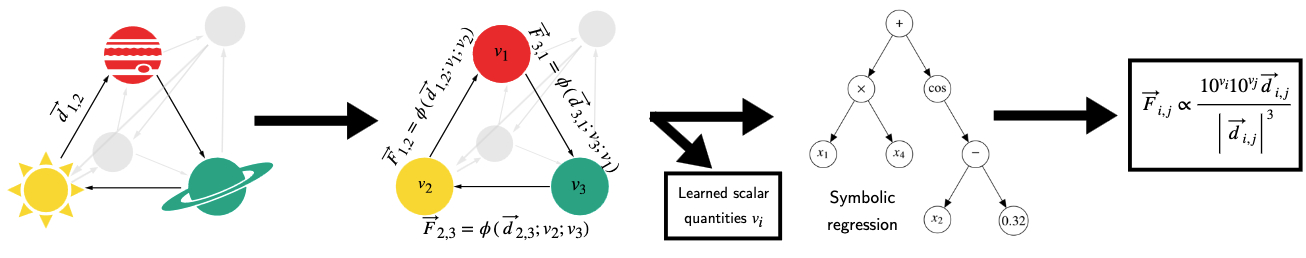
\includegraphics[width=200px]{img/retrieve_gravitation_laws_2.png}
  \end{textblock}
  \begin{textblock}{80}(4, 50)
    \begin{itemize}
      \item Based on GNN and symbolic regression
      \item Two-step approach: training a GNN-based simulator, then using symbolic regression to find analytical formulae for forces
      \item Loss function obtained by comparing this predicted acceleration and the true acceleration
    \end{itemize}
  \end{textblock}

  \note{By training a GN to simulate orbital
  dynamics from real data, authors say they were able to extract the edge function and correctly infer the formula
  for Newtonian gravitation.}

  \begin{textblock}{80}(4, 80)
    \begin{itemize}
      \item Do we want to automate Science? 
      \item What are the constraints and the theoritical limits? 
    \end{itemize}
  \end{textblock}

\end{frame}


\section{Conclusion}

% Challenges
\begin{frame}
  \note{
    \begin{itemize}
    \item Provide some insights on data hell
    %\item How would you rate GW data?
    \item Challenges in particular theoretical development
    \end{itemize}
  }
  \frametitle{Challenges}

  \begin{textblock}{90}(5, 10)
    \begin{itemize}
    \item Obtaining good data is hard:
      \begin{itemize}
      \item Challenges of ``big data'': volume, velocity, variety, veracity (4V)
      \item Systematic biases
      \item Legal issues: GDPR, sensitive research, confidentiality
      \item Data acquisition, cleaning and normalization can take up to 80\% of
        the time
      \end{itemize}
    \item \acl{xAI}:
      \begin{itemize}
      \item Opening the black-box
      \item Interpretability: begin able to build indicators on the decision of the model
        (which variables are the most important, understand parts of the model)
      \item Explicability: being able to explain the decision of the model
      \end{itemize}
    \item Ethical \ac{AI}:
      \begin{itemize}
      \item How to build systems which respect fundamental values like individual rights, privacy, non-discrimination and non-manipulation?
      \end{itemize}
    \item More technical challenges:
      \begin{itemize}
      \item Unsupervised learning
      \item New protocols: online learning, active learning
      \item Reproductibility
      \item Not just predict but \emph{understand} the data
      \end{itemize}
    \end{itemize}
  \end{textblock}
\end{frame}


\begin{frame}
  \frametitle{See you soon in Toulouse!}
  \begin{center}\LARGE AISSAI Workshop: Heterogeneous Data and Large Representation Models in Science\end{center}
  \begin{center}
\includegraphics[width=200px]{img/invitation.png}\end{center}
  
  \begin{center}\large from September 30 to October 3rd, 2024\end{center}
  \begin{center}\large \url{https://indico.in2p3.fr/event/33412/}\end{center}
  % \begin{center}\Large See you soon in Toulouse!\end{center}
\end{frame}


\appendix

% Appendices outline
\begin{frame}
  \frametitle{Appendices}
  \tableofcontents[hidesubsections]
\end{frame}

\AtBeginSection[]{%
  \begin{frame}
    \frametitle{Appendices}
    \tableofcontents[currentsection,subsectionstyle=show/shaded/hide]
  \end{frame}
}

\section{A bit more context}

\begin{frame}{A picture of the the Dartmouth workshop}
  \note{
    \begin{itemize}
    \item This is equivalent to the famous photo of the Solvay conference
    \end{itemize}
  }

  \begin{textblock}{90}(5, 10)
    \begin{center}
      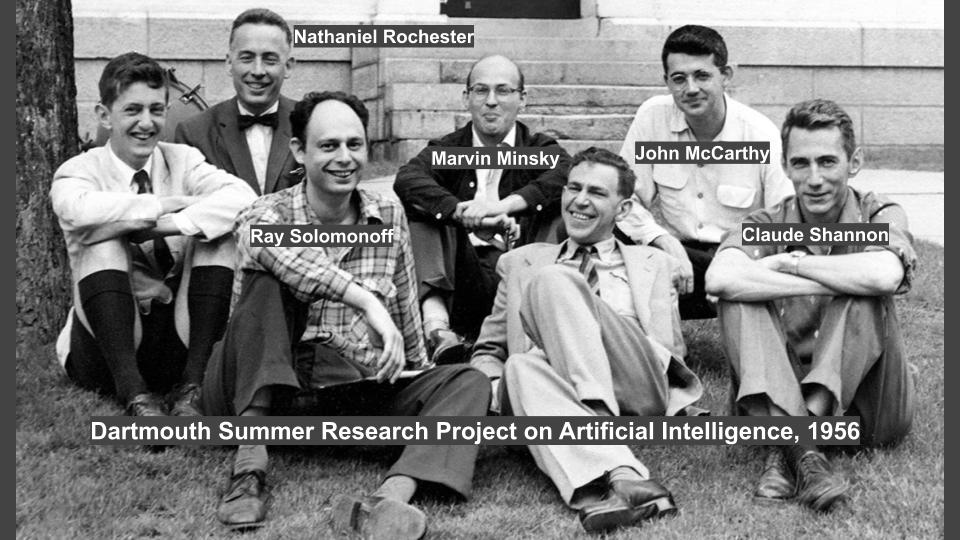
\includegraphics[height=4cm]{img/dartmouth-conference.jpg}
    \end{center}
  \end{textblock}

  \begin{textblock}{95}(5, 58)
    More or less full list of attendees:
    \begin{footnotesize}
    \begin{columns}[T]
      \begin{column}{0.33\textwidth}
        \begin{itemize}
        \item Ray Solomonoff
        \item Marvin Minsky
        \item John McCarthy
        \item Claude Shannon
        \item Trenchard More
        \item Nat Rochester
        \end{itemize}
      \end{column}

      \begin{column}{0.33\textwidth}
        \begin{itemize}
        \item Oliver Selfridge
        \item Julian Bigelow
        \item W. Ross Ashby
        \item W.S. McCulloch
        \item Abraham Robinson
        \item Tom Etter
        \end{itemize}
      \end{column}

      \begin{column}{0.33\textwidth}
        \begin{itemize}
        \item John Nash
        \item David Sayre
        \item Arthur Samuel
        \item Kenneth R. Shoulders
        \item Alex Bernstein
        \item Herbert Simon
        \item Allen Newell
        \end{itemize}
      \end{column}
    \end{columns}
  \end{footnotesize}
\end{textblock}
\end{frame}


% Present the important steps in a project
% Inspired by barra2006, chapter 2, section 1
\begin{frame}
  \frametitle{Steps in a \ac{ML} project}

  \begin{textblock}{90}(5, 15)
    \begin{enumerate}
      % 1.1.1 and 1.1.3
    \item Get familiar with the application domain and the type of data
      % 1.1.2
    \item Get the data and clarify input \& output of each step
      % 1.1.4
    \item Clean and normalize the data
      % 1.1.5
    \item Explore data:
      \begin{itemize}
      \item Descriptive statistics
      \item Visualization
      \end{itemize}
      % 1.1.7 (and 1.1.6)
    \item Compare various methods:
      \begin{itemize}
      \item Take into account the technical limits (computational power \&
        storage, \etc{})
      \item Establish a baseline (``classic method'') and compare other methods
        to it
      \end{itemize}
      % 1.1.8 and 1.1.9
    \item Optimize and evaluate the method
    \item Deploy \& monitor the solution:
      \begin{itemize}
      \item Might require a different implementation to face run time constraints
      \end{itemize}
    \end{enumerate}
  \end{textblock}
\end{frame}


% Appendices
% To be used with hyper links

\begin{frame}[label=Backpropagation]
  \frametitle{\acl{MLP}: Compute the gradient (1/2)}

  \begin{textblock}{90}(5, 15)
    \begin{itemize}
    \item Gradient:
      $
      \grad_{\params} \apply{\lossFunc}{\apply{\hyp_{\params}}{\example_i}, \knownLabel_i} =
      \left( \partialDeriv{\apply{\lossFunc}{\apply{\hyp_{\params}}{\example_i},
            \knownLabel_i}}{w_{1,1}^1}, \ldots, \partialDeriv{\apply{\lossFunc}{\apply{\hyp_{\params}}{\example_i}, \knownLabel_i}}{w_{k,p}^l},\ldots,\partialDeriv{\apply{\lossFunc}{\apply{\hyp_{\params}}{\example_i}, \knownLabel_i}}{w_{N_{4},N_{3}}^{3}} \right)^T
      $

      \begin{itemize}
      \item Analytical calculation is possible but tedious
      \end{itemize}
    \item $\hyp_{\params}$ is a composition of functions:
      \[
        \apply{\hyp_{\params}}{\example} = \apply{\softMaxFunc}{%
          \weightMatrix^3 \times
          \apply{\ReLUFunc}{%
            \weightMatrix^2 \times
            \apply{\ReLUFunc}{%
              \weightMatrix^1 \times \example
            }
          }
        }
      \]
      \begin{itemize}
      \item Use the chain rule to compute partial derivatives.
      \end{itemize}
    \end{itemize}
  \end{textblock}
\end{frame}

\begin{frame}
  \frametitle{\acl{MLP}: Compute the gradient (2/2)}

  \begin{textblock}{90}(5, 15)
    \begin{block}{Derivation of the gradient}
      \begin{itemize}
      \item Apply the chain rule at layer $\ell$:
        $
        \partialDeriv{\apply{\lossFunc}{\apply{\hyp_{\params}}{\example_i}, \knownLabel_i}}{w_{k,p}^\ell} =
        \partialDeriv{\apply{\lossFunc}{\apply{\hyp_{\params}}{\example_i}, \knownLabel_i}}{o_k^{\ell+1}} \partialDeriv{o_k^{\ell+1}}{s_k^{\ell+1}} \partialDeriv{s_k^{\ell+1}}{w_{k,p}^{\ell}}
        $

      \item $\partialDeriv{\apply{\lossFunc}{\apply{\hyp_{\params}}{\example_i}, \knownLabel_i}}{o_k^{\ell+1}}$: known at the $\ell+1$ layer. $\partialDeriv{\apply{\lossFunc}{\apply{\hyp_{\params}}{\example_i}, \knownLabel_i}}{o_k^{L}}$: last layer, $\lossFunc$ must be differentiable w.r.t $o_k^{L}$.

    %\item $\partialDeriv{\apply{\lossFunc}{\apply{\hyp_{\params}}{\example_i}, \knownLabel_i}}{o_k^{L}}$: last layer, $\lossFunc$ must be differentiable w.r.t $o_k^{L}$

      \item $\partialDeriv{o_k^{\ell+1}}{s_k^{\ell+1}}$: $o_k^{\ell+1} = \activFunc(s_k^{\ell+1})$, $\activFunc$ as intermediate or final activation function must be differentiable.

      \item $\partialDeriv{s_k^{\ell+1}}{w_{k,p}^{\ell}} = \partialDeriv{}{w_{k,p}^{\ell}} \sum_{p' \in \left\{1,\ldots,N_l \right\}}  w_{p', k}^{\ell}o_{p'}^{k}= \partialDeriv{}{w_{k,p}^{\ell}}  w_{p, k}^{\ell}o_{p}^{\ell}=o_{p}^{\ell}$

    \end{itemize}
    \end{block}
  \end{textblock}

  \begin{textblock}{90}(5, 65)
    \begin{block}{General idea}<2->
      \begin{itemize}
      \item Back-propagation works for all feed-forward architectures
        \hyperlink{MLP_Learning_2}{\beamergotobutton{Go back}}
        % Back-propagates to main slide :)
      \end{itemize}
    \end{block}
  \end{textblock}
\end{frame}


%% Appendices
% To be used with hyper links

\begin{frame}[label=Convolutional_Layers]
  \frametitle{\acl{CNN}: Convolutional Layers}

  \begin{textblock}{90}(5, 10)
    \begin{center}
      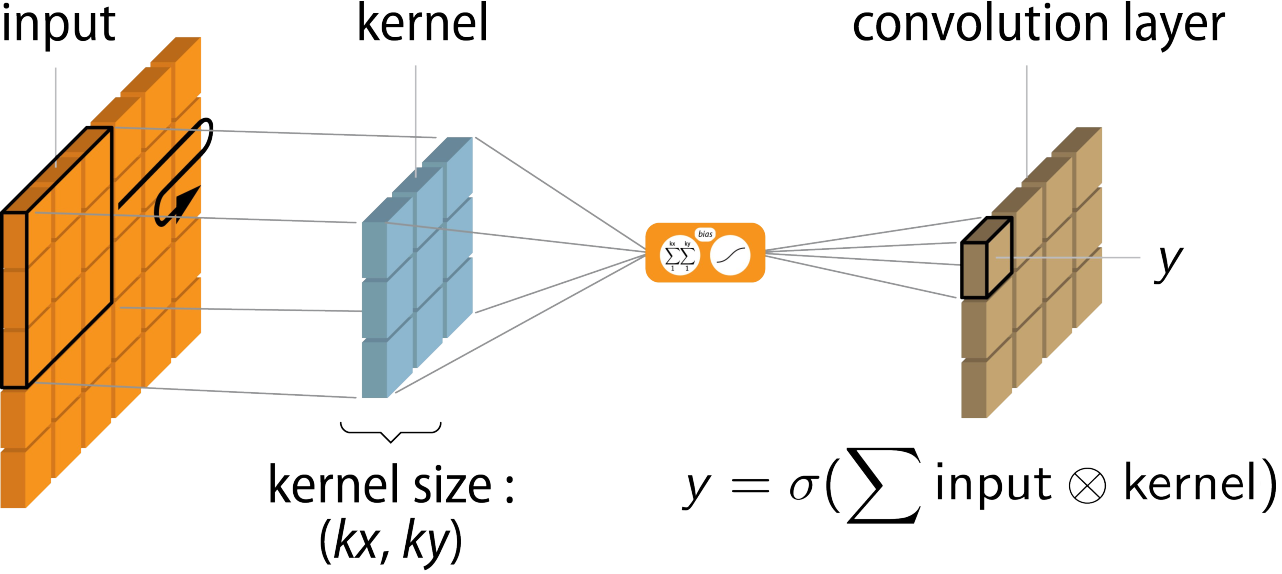
\includegraphics[width=\textwidth]{img/Convolution.png}
      Taken from FIDLE
    \end{center}
  \end{textblock}

  % Cheat a bit on the size
  \begin{textblock}{46}(5, 75)
    \begin{itemize}
    \item Common operation in image processing
    \item $\matrix{K}$ acts as a filter
    \end{itemize}
    \hyperlink{CNN_Overview_Convolutional}{\beamergotobutton{Go back}}
  \end{textblock}

  \begin{textblock}{45}(50, 75)
    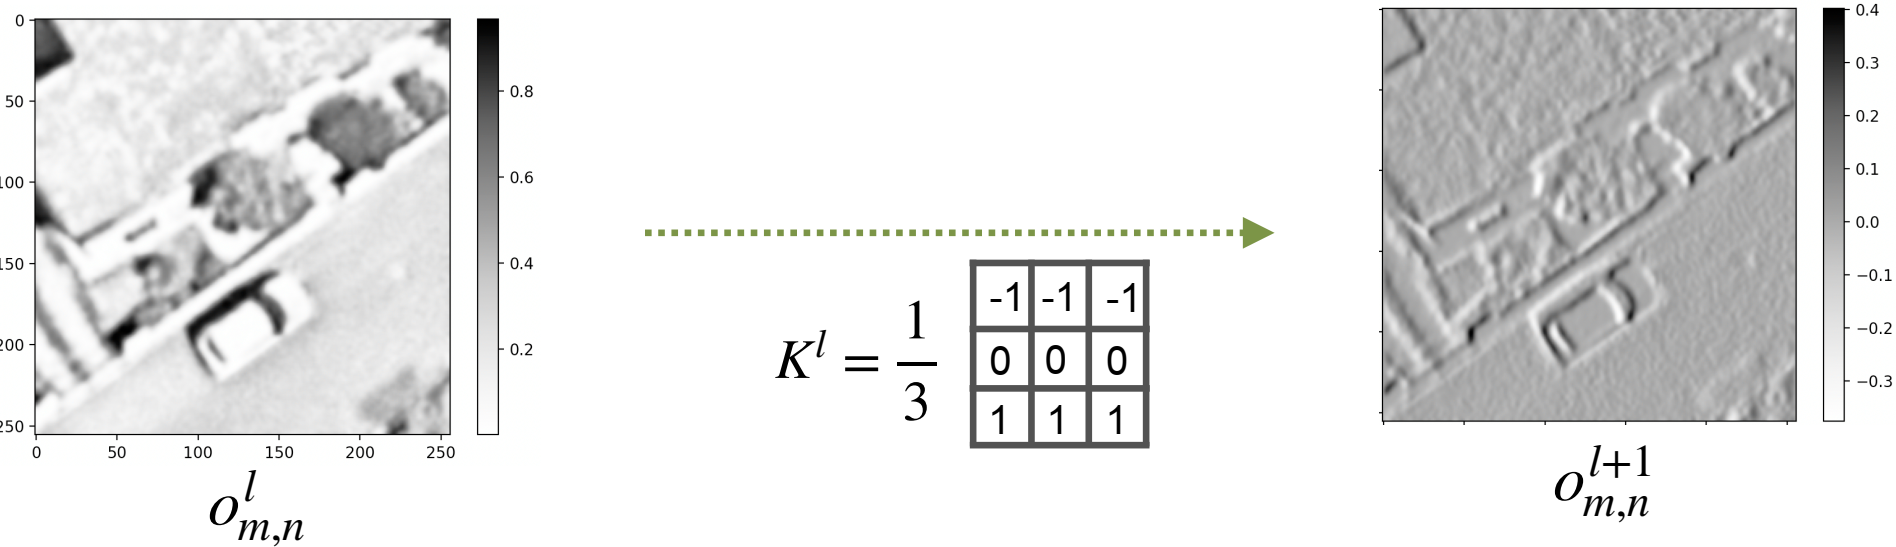
\includegraphics[width=\textwidth]{img/CNN_Filter.png}
  \end{textblock}
\end{frame}


\begin{frame}[label=Pooling_Layers]
  \frametitle{\acl{CNN}: Pooling Layers}

  \begin{textblock}{90}(5, 10)
    \begin{center}
      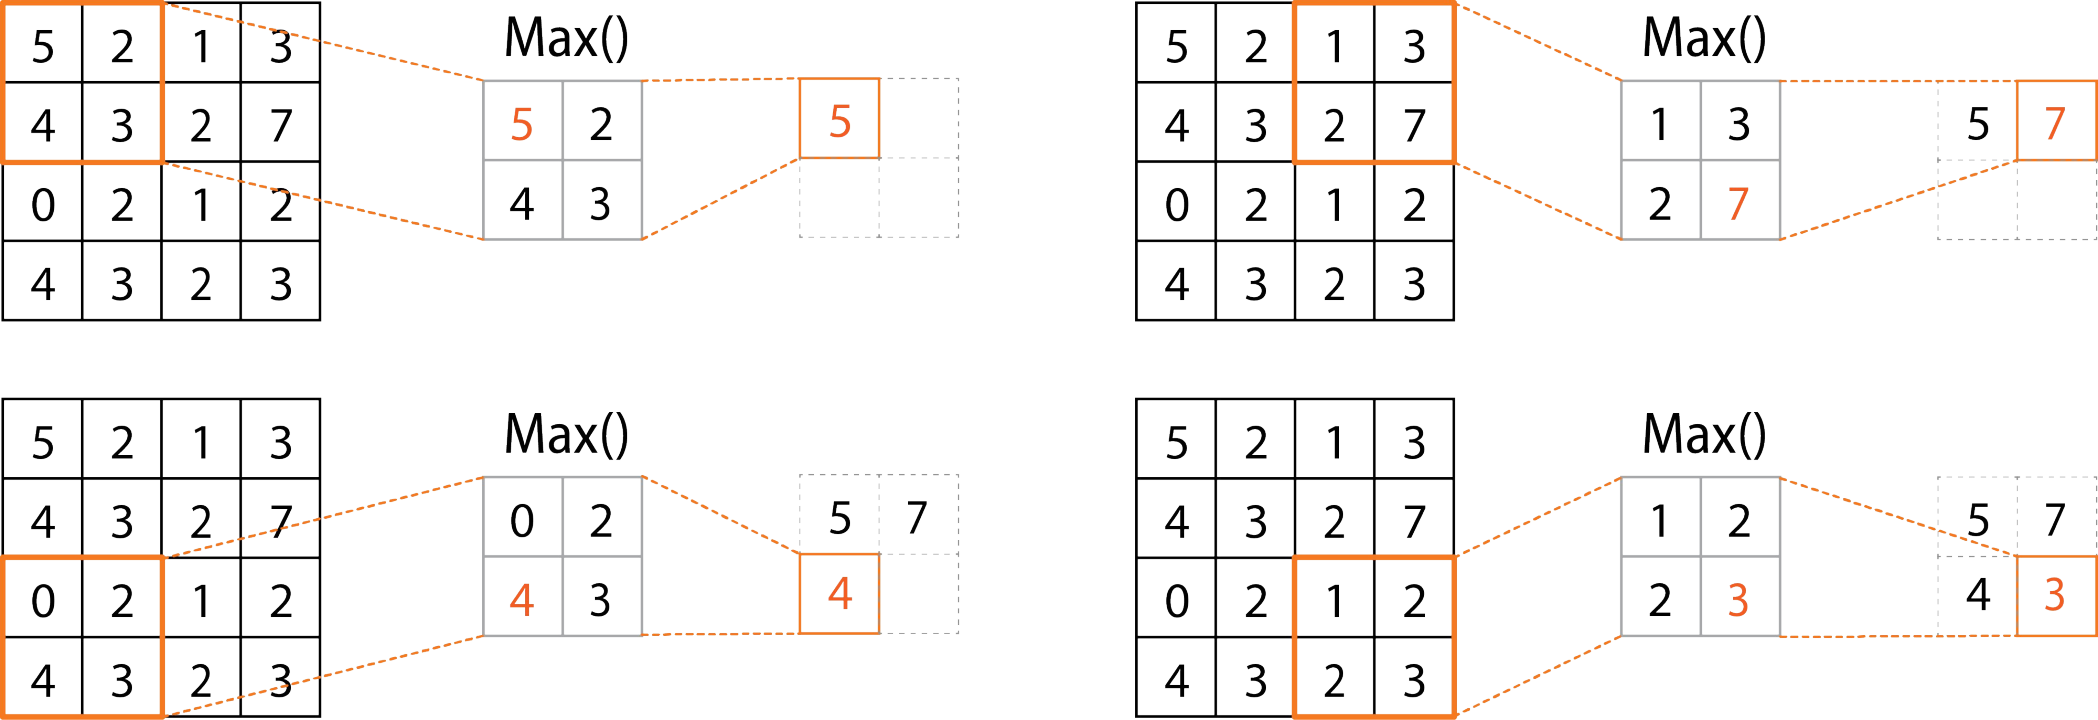
\includegraphics[width=\textwidth]{img/CNN_Pooling.png}
      Taken from FIDLE
    \end{center}
  \end{textblock}

  \begin{textblock}{90}(5, 75)
    Crude downsampling (dimensionality reduction)\\
    \hyperlink{CNN_Overview_Pooling}{\beamergotobutton{Go back}}
  \end{textblock}
\end{frame}


\end{document}
